\documentclass[oneside]{article}
\usepackage{fullpage}
\usepackage[pdftex]{graphicx}
\DeclareGraphicsExtensions{.png,.pdf}
\graphicspath{{images/}}
\usepackage{hyperref}
\usepackage{verbatim}
\usepackage[format=plain,font=small]{caption}
\usepackage[small]{titlesec}
\usepackage[round,sectionbib]{natbib}
\usepackage{amstext}
\bibliographystyle{plainnat}
\renewcommand\rmdefault{bch}
\linespread{1.07} 

\newcommand\amin{\text{minor}}
\newcommand\amaj{\text{major}}

\begin{document}

\title{Glyph-maps for Visualizing Climate Data and Models}
\author{Hadley Wickham$^1$, Heike Hofmann$^2$, Charlotte Wickham$^2$, Dianne Cook$^2$\\
$^1$ Department of Statistics, Rice University}
$^2$Department of Statistics, Iowa State University\\
$^3$ Department of Statistics, Oregon State University\\
\date{}

% Remove words like "obvious", "challenge", "scratched the surface"
% Make data URLs references
% Do we have different aspect ratios between the different US maps?
% Check where data is described, just use key names given in the description at beginning of paper

% Found data: http://www.esrl.noaa.gov/psd/data/gridded/data.HADCRUT2.html
%     air.mon.anom.nc, var adj, this is 5x5 degree grid, a bit sparse
% Or: http://www.esrl.noaa.gov/psd/data/gridded/data.gisstemp.html
% air.2x2.mon.anom.land.nc 250k smooth data, is on a 2x2 grid

% Drawing trend lines on map
%   - How to
%   - Comparison to coloring slope
%   - Reference to Grinstein icon plots
% Pickett RM and Grinstein GG (1988). Iconographics 
% displays for visualizing multidimensional data. 
% In Proc. IEEE Conference on Systems, Man, and Cybernetics, pages 514-19.
% Note the later work on metaphoric data display, garbage work!
%   - Alexander Gribov's work http://rosuda.org/software/Gauguin/gauguin.html

%   - Spatial star plots by Andrews http://www.udallas.edu:8080/~andrews/software/software.html
%   - Look at what Bertin does
%
% Interactive graphics
% Data processing
%
% Perhaps the GHCN data? Not gridded
% NOAA data, almost grid, but over ocean, so maps more tricky
% NARCAP from NCAR?
% Fill in with NASA data, to start, try to put new data for final version
\maketitle

\begin{abstract}

Climate data is challenging to visualize because it is multivariate and has both spatial (2d) and temporal (1d) components. In this paper we propose an new display for climate data: glyph-maps. Glyph-maps are a specialization of multivariate glyph plots; each spatial location is display with one glyph that represents the measurements recorded over time at that location. Glyph-maps allow the discovery of both local and global structure, making discovery much easier than the classical display using colors.

We include a description of how to create glyph-maps using existing statistical software, our initial explorations of their perceptual features, and a discussion of reference frames. Our techniques are inspired by rectangular gridded data, but we provide generalization to deal with non-rectangular grids and irregular locations.

\end{abstract}

\section{Introduction}

Climate data is composed of measurements, such as temperature, precipitation, and winds, with a spatial and temporal context. The classic display for data of this type of is ``heatmap'', a tiled plot using color to display the value of the variable of interest as each location. When measurements are made at multiple time points it is common to display the data with small multiples, such as in Figure~\ref{fig:nasa-facet}. In this plot, a separate map is drawn for each month (columns) and year (rows), over a 6 year period of remotely sensed temperature data above Central America \citep{murrell:2010}. Color is used to display de-seasonalized temperature, with red mapped to high values and blue to low. The most noticeable feature is the strong red patch in the equatorial Pacific beginning mid-1997 and tapering out during 1998. This is the El Ni\~no event, a major temperature anomaly. More work is required to see more localized patterns, like the cooler land temperatures seen in early years.

Reading this type of plot is cognitively challenging: the reader must play ``spot the difference'' from one small image to another. Large structures such as El Ni\~no are clear but it is very difficult to mentally difference the images and read off the long-term trend or to notice local deviations. Using a movie to render these small multiples can help, but small trends still fail to draw readers' attention and escape unnoticed \citep{simons:gradual}.

\begin{figure*}[htbp]
  \centering
  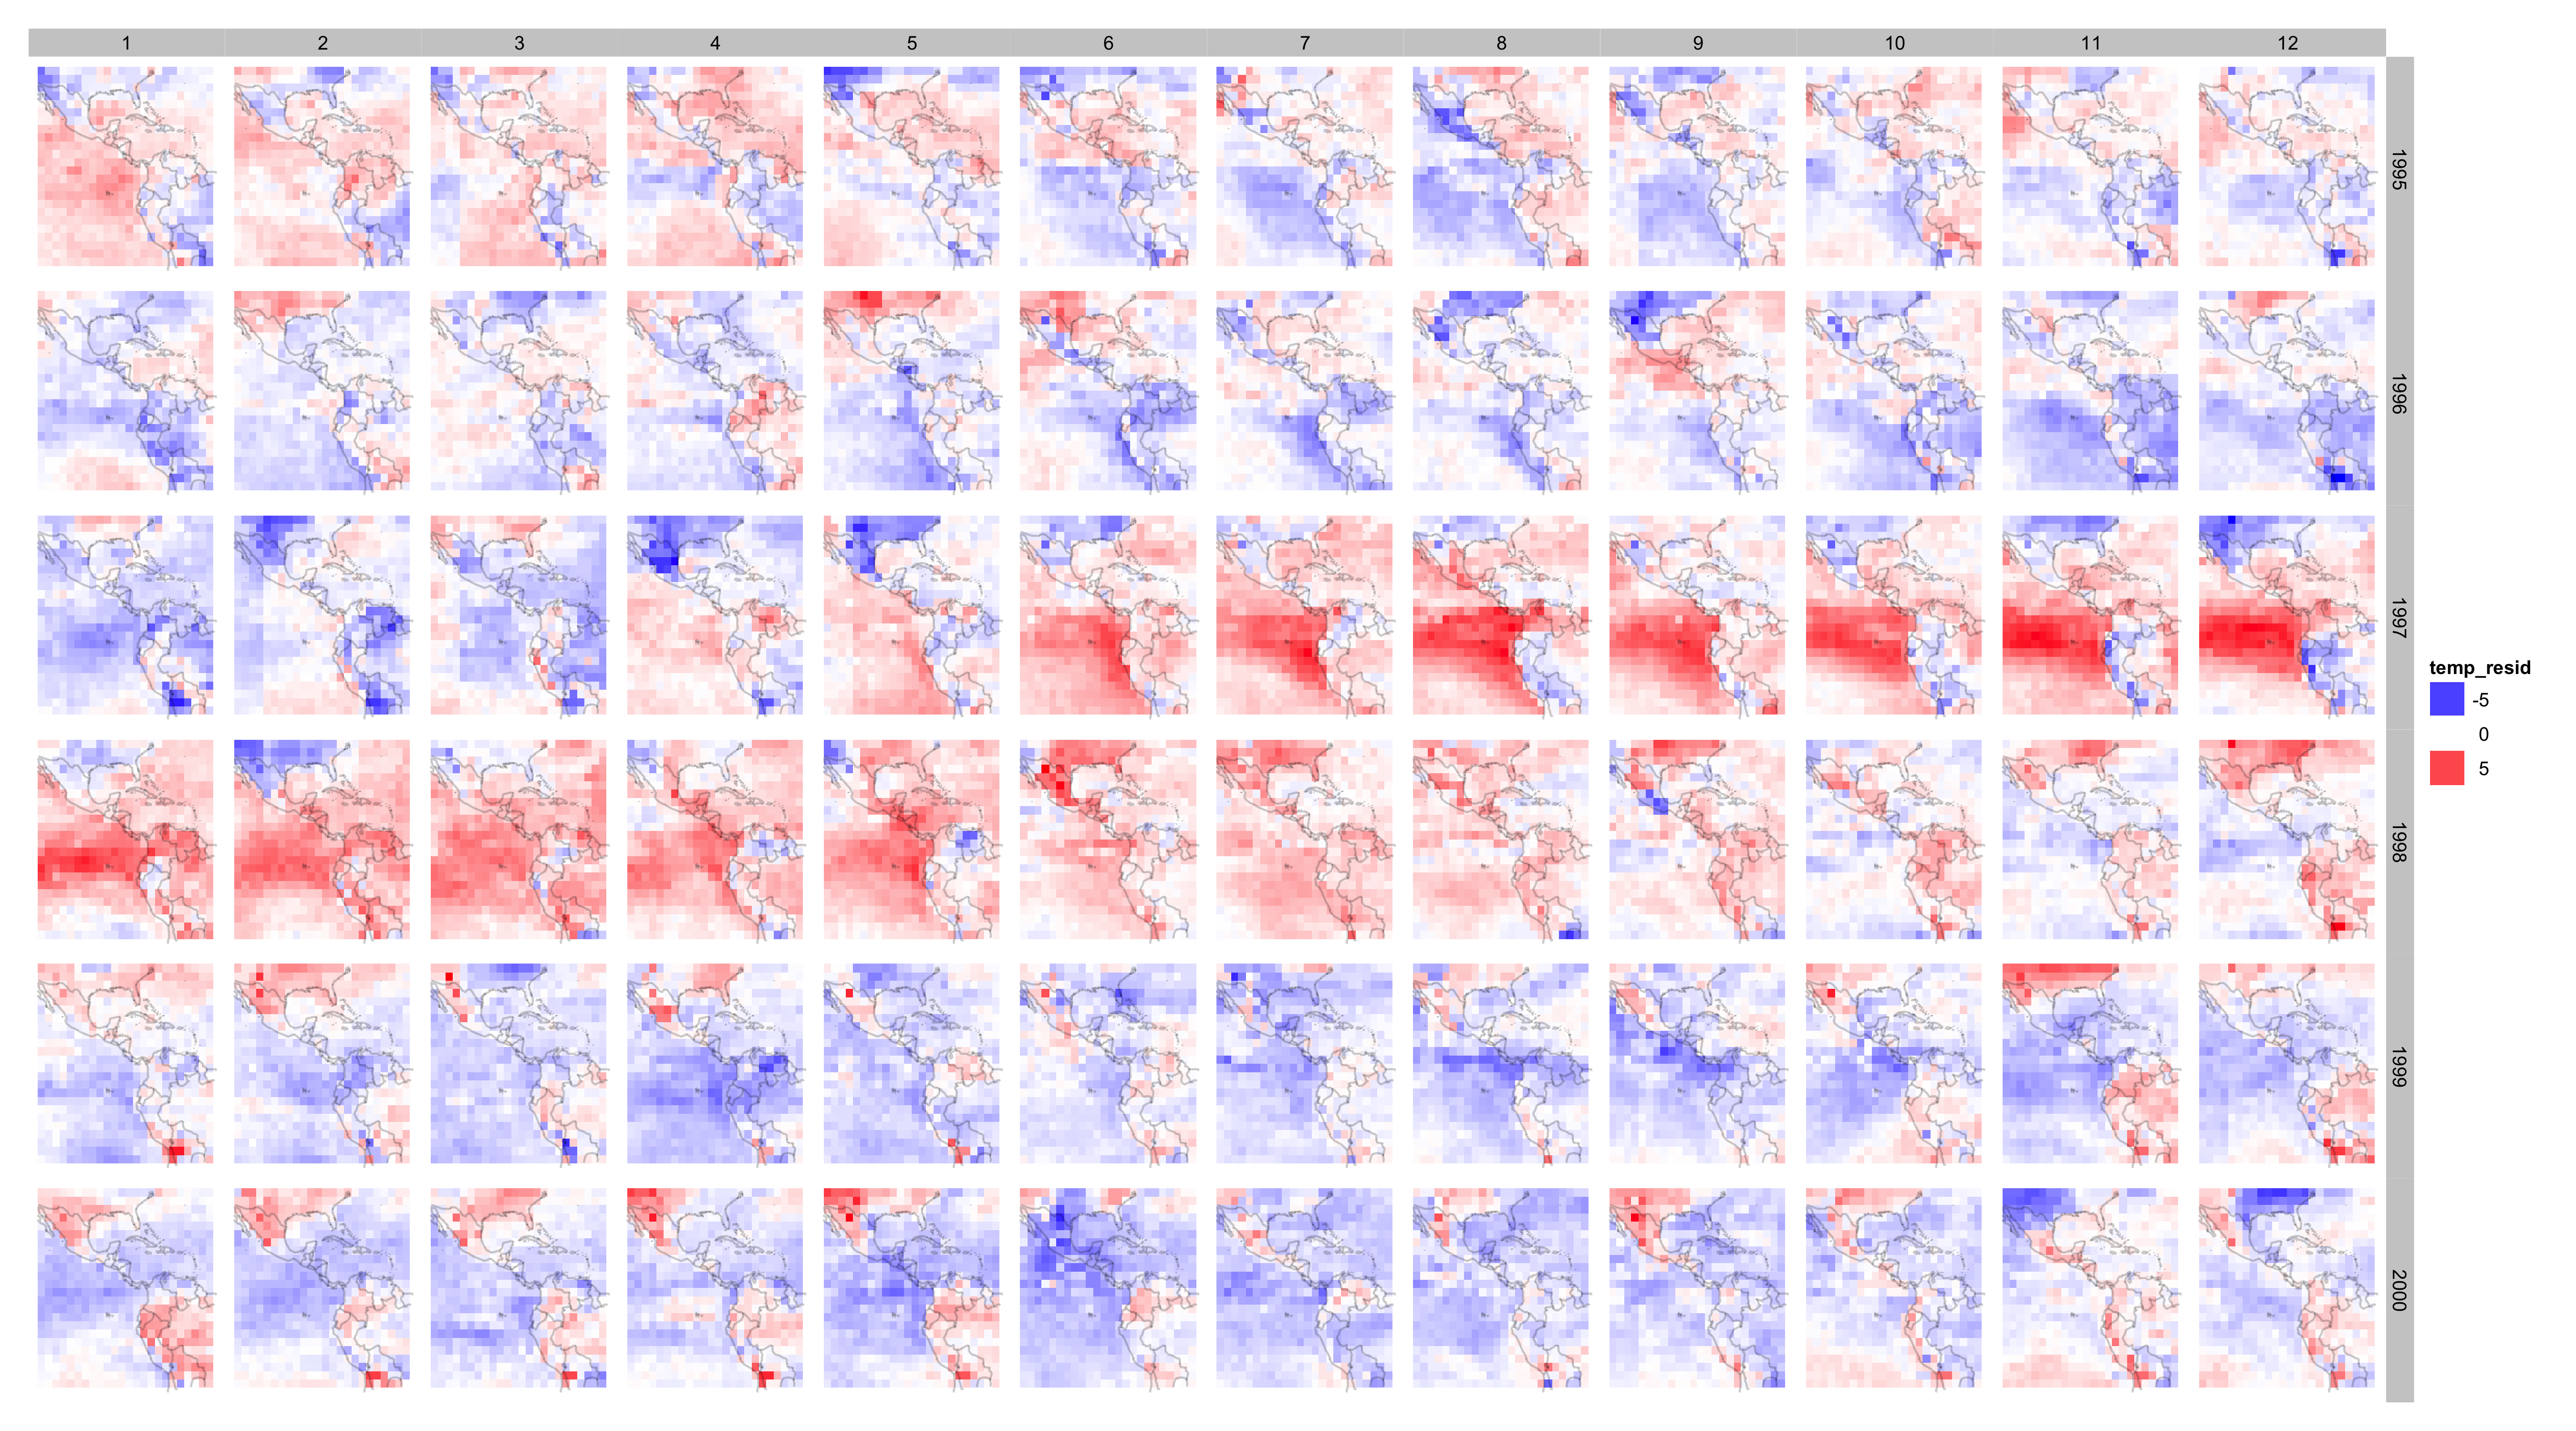
\includegraphics[width=5.5in]{nasa-colored-map.png}
  \caption{Facetted map of de-seasonalized temperature. The dominant feature is the El Ni\~no warming in the southern equatorial region in the last half of 1997 and first half of 1998. Smaller features are only noticeable on closer inspection, or if pointed out: such as the relative warming on the mountain regions in south and north America in the later years.}
  \label{fig:nasa-facet}
\end{figure*}

\begin{figure*}[htbp]
  \centering
  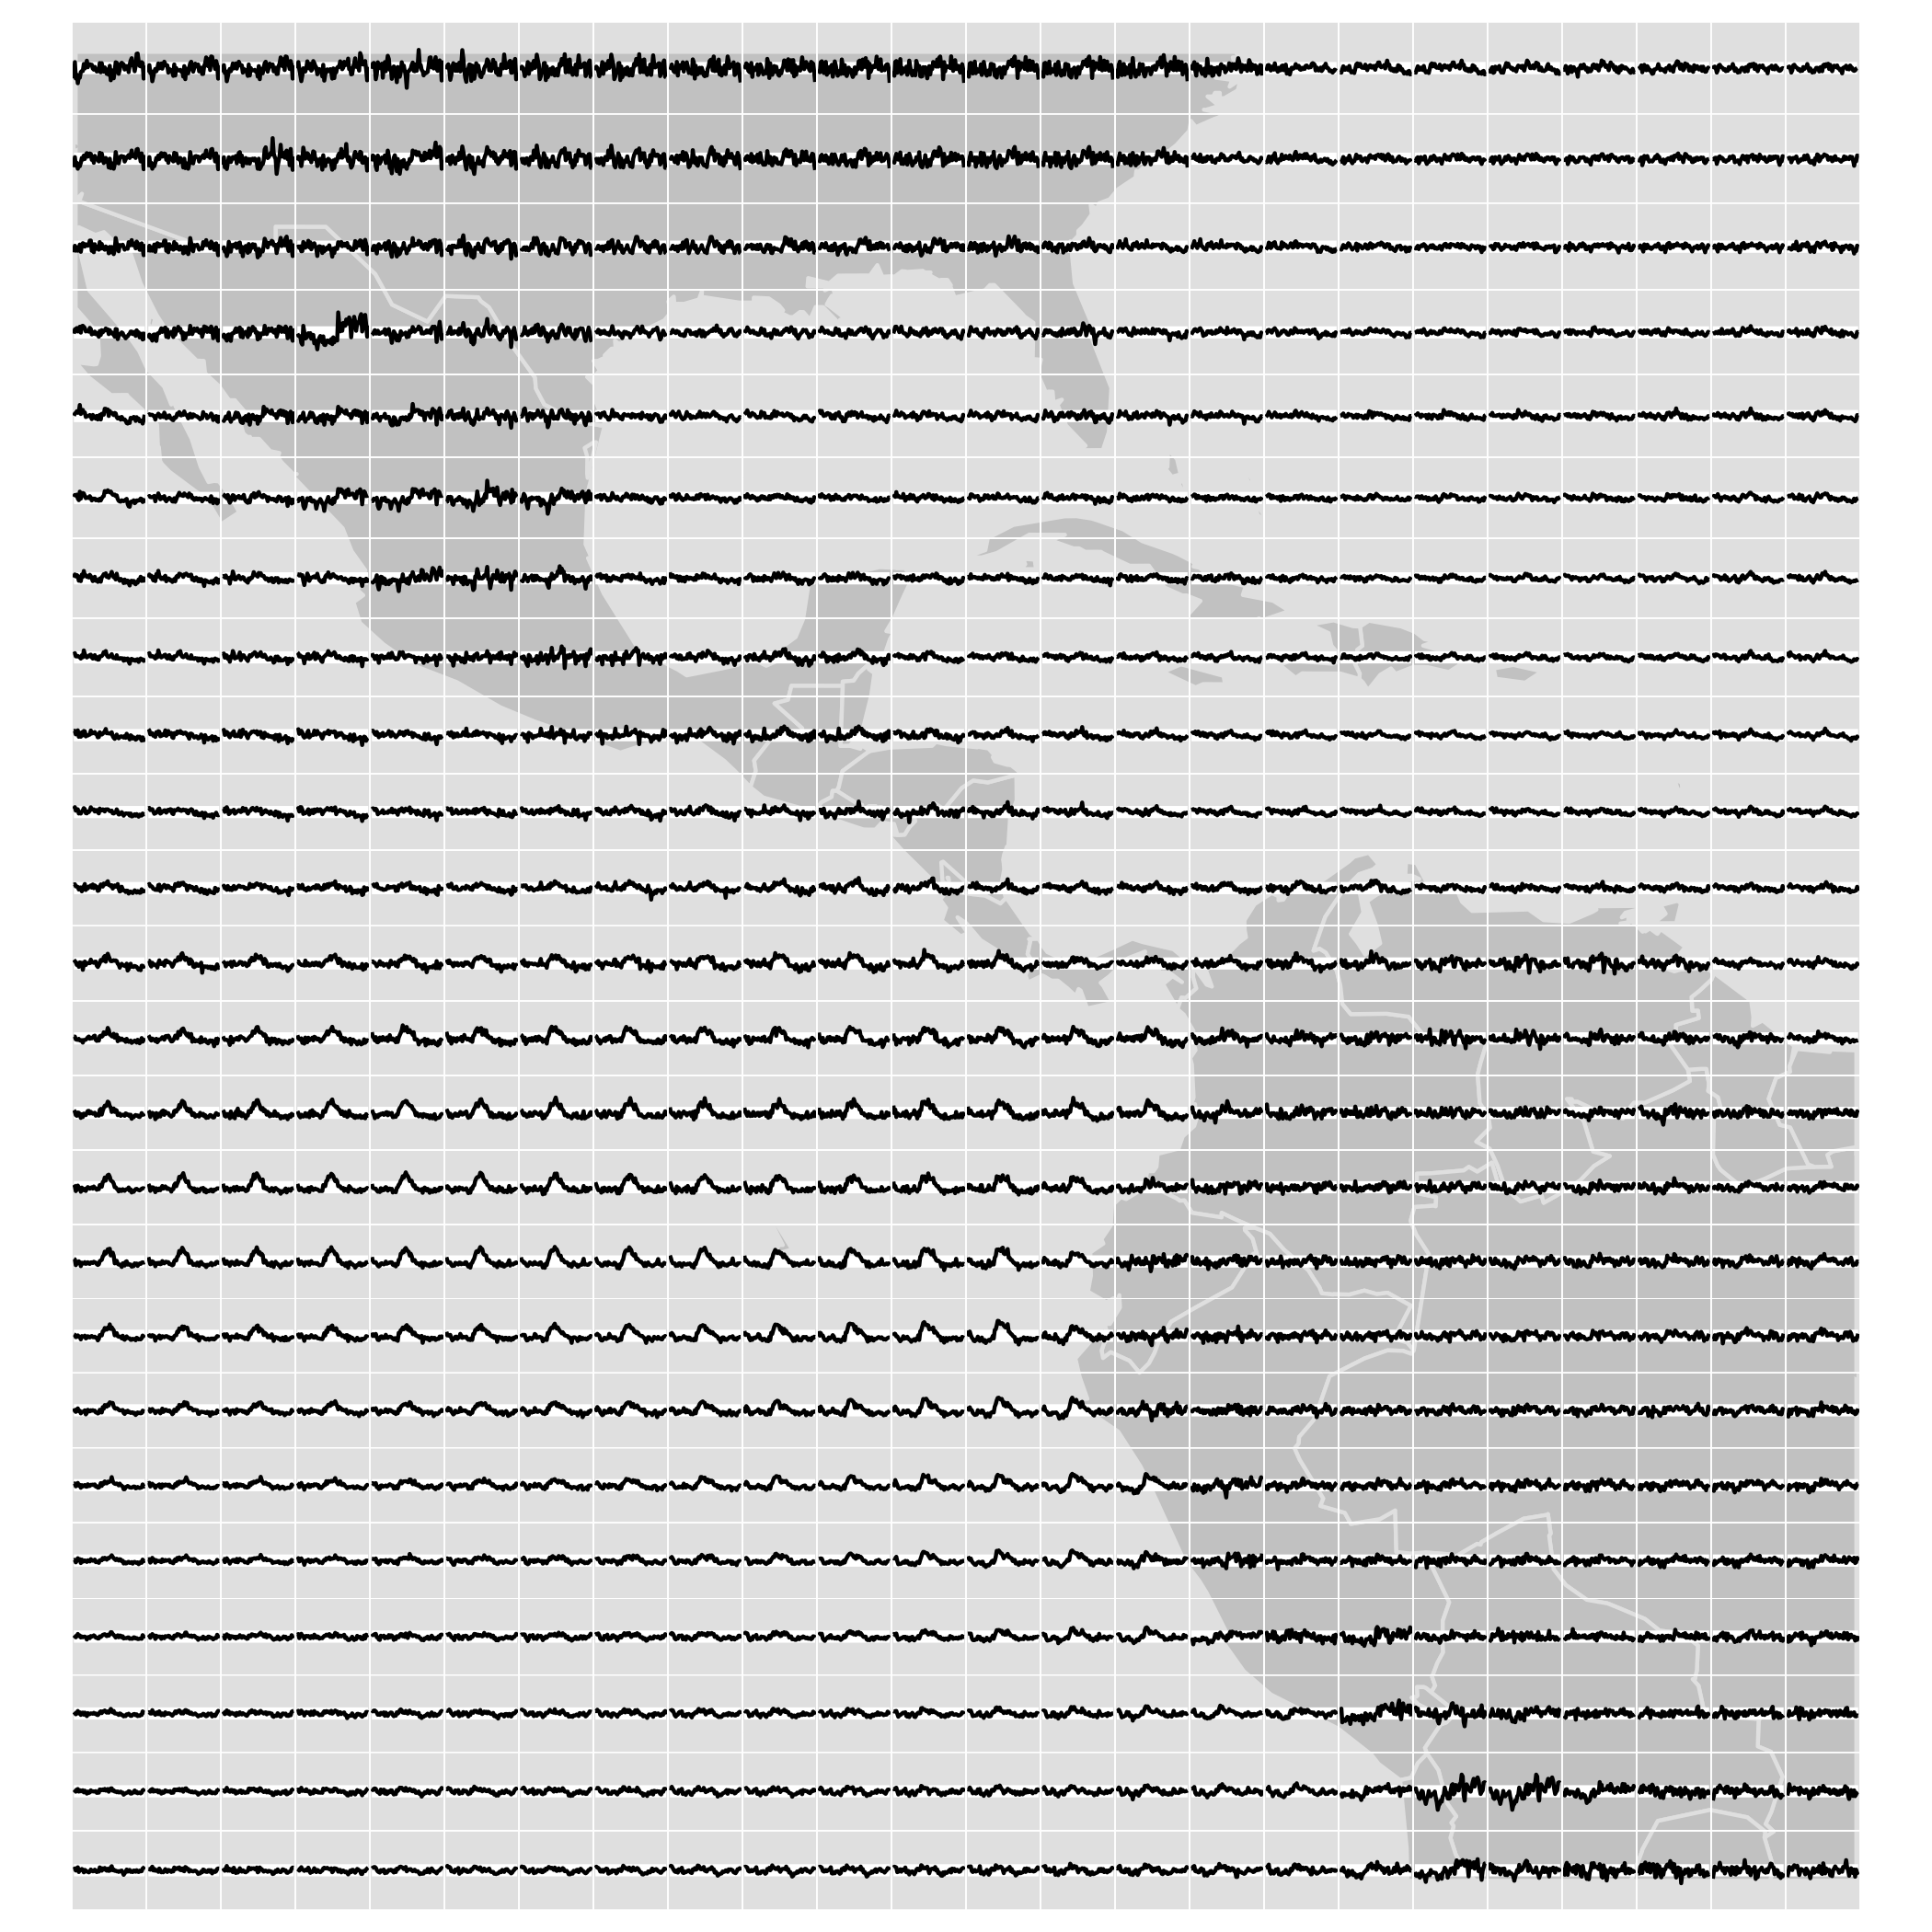
\includegraphics[width=3.5in]{nasa-deseas-glyph}
  \caption{Glyph-map of de-seasonalized temperature, to compare with Figure \ref{fig:nasa-facet}. Time series of the six years of monthly temperature are plotted at each spatial grid location. The El Ni\~no appears as a bump in the middle of the time series, in the equatorial Pacific region. Large variations in temperature can be seen in areas over land, while being fairly constant over water. }
  \label{fig:nasa-glyph}
\end{figure*}

%% Reproduce all of the icon displays using the fixed glyph code

In this paper we develop a new type of display to resolves these problems: the \emph{glyph-map}. The glyph-map uses a small glyph, or icon, to represent multiple values at each location. Glyph maps are an adaptation of glyphs, tools developed for display multivariate data. Multivariate glyphs include the star plots of \citet{mayr:1877}, the semi-graphic displays of \citet{anderson:1960}, and the infamous Chernoff faces \citep{chernoff:1973}. An glyph is produced by mapping each variable to some graphical feature, such as the length of a line. The glyph-map can also be thought of as a small multiple display \citet{tufte:2001} of time series with a geographic context.

Figure~\ref{fig:nasa-glyph} shows the glyph-map equivalent of Figure~\ref{fig:nasa-facet}: each location is represented by a small time series glyph. The primary visible structure is still El Ni\~no, the regions in the Pacific with bump in the middle of the series, but we can also see other features: temperatures are generally more varied over land and a few locations have dramatically increasing temperature in the later years typically in high elevation areas, along the Andes and the Sierra Madre Occidental in Mexico.

% The most seasonality occurs in north American. Some seasonal effects can also be seen in the Caribbean and in south American locations. Around the equator the temperatures are relatively warm for all seasons. Instead of radially displaying the temperature a glyph can be a regular time series, time displayed horizontally and temperature vertically (right plot). The structure perceived is different with this change in glyph type: locations at the equator have flat series, on land more varied temperatures. 

One problem with multivariate glyph is that lack of natural ordering of each glyph, or of the mapping between variables and glyph properties. This leads to a combinatorial explosion of possibilities, each of which may have dramatically different perceptual properties. This problem has prevented the widespread adoption of glyph displays, despite some proposed remedies \citep{kleiner:1981,hurley:2010}. Using glyphs with space-time data makes the problem go away: we place glyphs according to the location of the measurement, and we order variables by the time they were collected. Additionally, climate data usually has high correlations between nearby locations and times. This imposes a degree of smoothness that gives the plot an appearance of a textured  landscape, making it easier to digest patterns. Others \citet{pickett:1988} have used glyphs on maps to display multivariate spatial data. This area of work has morphed into the field of metaphorical data displays, which creates abstract landscapes of spatial data, a digression from glyph-maps. \citet{gribov:2006} describes the use of glyph-maps for multivariate data also, with emphasis on the graphics software Gauguin.

We focus our attention on two types of glyph: lines and stars. Figure~\ref{fig:templates} displays 12 iconic time series shapes with line- and star-glyphs. The data underlying each glyph is measured at 36 time points. The line-glyphs are a simple time series plot. The star-glyphs are formed by considering the 36 axes radiating from a common midpoint, and the data values for the row are plotted on each axis relative to the locations of the minimum and maximum of the variable. This is a polar transformation of the line-glyph.

\begin{figure}[htbp]
  \centering
  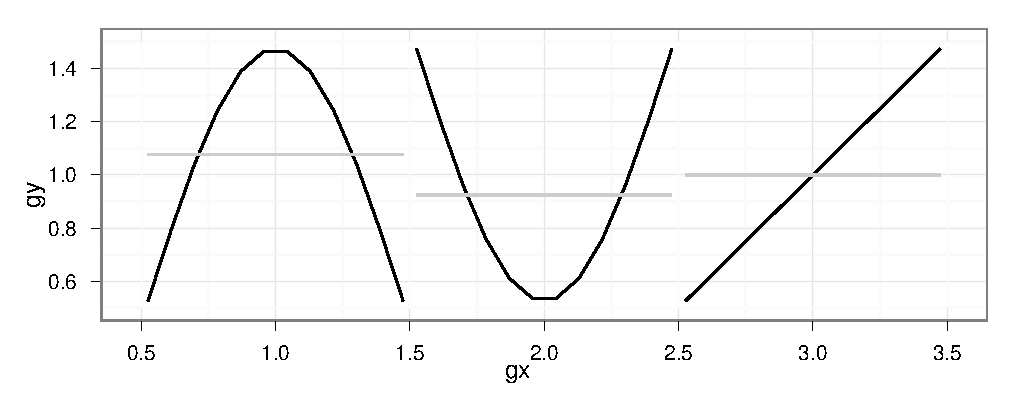
\includegraphics[width=0.5\linewidth]{euclid-to-polar-1}%
  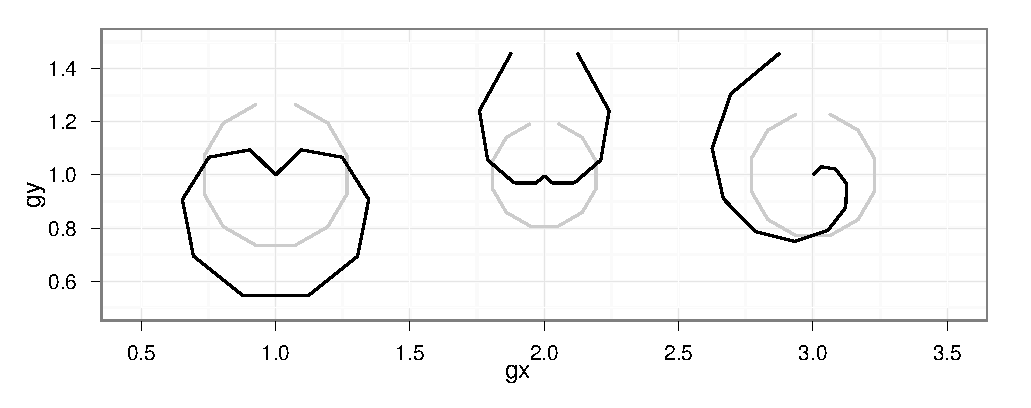
\includegraphics[width=0.5\linewidth]{euclid-to-polar-2}

  \caption{Icon plots for 12 iconic time series shapes (linear increasing, decreasing, shifted, single peak, single dip, combined linear and nonlinear, seasonal trends with different scales, and a combined linear and seasonal trend) in Euclidean coordinates, time series icons (left) and polar coordinates, star plots (right).}
  \label{fig:templates}
\end{figure}

%Glyph-maps have attributes of both glyphs (stars, faces, profiles, ...), inviting exploration at the global level, and small-multiple time series, allowing local exploration of individual series. Allow to see both geographic context and individual locations simultaneously.

%These displays tend to be particularly effective when printed in large format, as the much higher resolution of print (600 dpi) compared to computer  screen (72-120 dpi) allows for much finer reading. These are high-density data displays in the best tradition of Tufte. Wall size maps are not usually practical during analysis, but are very engaging.

We begin in Section~\ref{sec:construction} by describing the algorithm used to create glyphs-maps. Section~\ref{sec:perception} discusses their perceptual properties, including the importance of a visual reference grid, and of carefully considering scale. Section~\ref{sec:large-data} shows how glyph-maps scale to large data, and the interplay of models with glyph-maps. We originally developed glyph-maps for data on a rectangular grid, but many spatiotemporal data sets have irregular spatial locations. Section~\ref{sec:irregular} discusses how glyph-maps can be adjusted for this type of data.

To demonstrate the glyph-map we will use three datasets:

\begin{itemize}

  \item The ASA 2009 data expo data which consists of monthly observations of
  several atmospheric variables from the International Satellite Cloud
  Climatology Project. The dataset includes observations over 72 months
  (1995--2000) on a 24 x 24 grid (576 locations) stretching from
  $113.75^{\circ}$W to $56.25^{\circ}$W longitude and $21.25^{\circ}$S to
  $36.25{^\circ}$N latitude.

\item GISTEMP surface temperature data provided on $2^{\circ}$ x
  $2^{\circ}$ grid over the entire globe, measured monthly. Ground
  station data was de-seasonalized, differenced from from the
  1951-1980 temperature averages, and spatially averaged to obtain
  gridded measurements. For the purposes of this paper, we extracted
  the locations corresponding to the continental USA. The data is made
  available by the Earth System Research Laboratory, Physical Sciences
  Division, National Oceanic and Atmospheric Administration, from
  their web site at \url{http://www.esrl.noaa.gov/psd/}.

  \item USHCN (Version 2) ground station network. USHCN data provided by NOAA NCDC from their website \url{http://cdiac.ornl.gov/ftp/ushcn_v2_monthly/}.
  
\end{itemize}

All datasets and R code used to produce the plots are available in the online supplementary materials. All plots were created in R \citep{R} using the {\tt ggplot2} \citep{me:ggplot2} and {\tt plyr} \citep{me:plyr} packages. 

\section{Construction}~\label{sec:construction}

Glyph-maps can be generated with existing graphics software after performing a simple pre-processing step, making them easily accessible to a wide audience. Creating a glyph-map requires a recognition they combine two structural components of the data: spatial location and data values. The spatial location is the major positioning component, and the data values are minor adjustments to those positions. For spatiotemporal data, the major axes are latitude ($y_{\amaj}$) and longitude ($x_{\amaj}$), and the minor axes are time ($x_{\amin}$) and some measurement ($y_{\amin}$), for example, temperature, or predicted temperature. Assuming the minor axes are rescaled to $[-1, 1]$, the final positions are a simple linear combination:

\begin{equation}
  \begin{array}{lll}
  x_\text{ coordinate}&=& x_{\amaj} + w \cdot x_{\amin}\\
  y_\text{ coordinate}&=& y_{\amaj} + h \cdot y_{\amin}, 
  \end{array}
  \label{coords.eqn}
\end{equation}

\noindent where $w$ and $h$ are width and height respectively. For gridded data, the width and height be the resolution of the major axes, that is, the minimum difference between consecutive locations. Since the coordinates are linear combinations of two variables, it is possible to build these these line-glyphs interactively, illustrated by software packages that have incorporated tours \citep{cook:2006}, such as DataViewer \citep{buja:1986}, XGobi \citep{swayne:1991} or GGobi \citep{swayne:2003}. This technique is used to good effect in \citet{buja:1996a}, and was used to examine the climate data in \citet{hobbs:2010}.

Computing the coordinates for star glyphs is achieved with a simple polar transformation, with minor axes scaled to $[0, 1]$: 

\begin{equation}
  \begin{array}{lll}
  x_\text{ coordinate}&=& x_{\amaj} + y_{\amin} \cdot \frac{w}{2} \sin(2 \pi x_{\amin}) \\
  y_\text{ coordinate}&=& y_{\amaj} + y_{\amin} \cdot \frac{h}{2} \cos(2 \pi x_{\amin}).
  \end{array}
  \label{coords.polar.eqn}
\end{equation}

\noindent This is a non-standard conversion to polar coordinates, but it creates a timeline that starts at 12 o'clock and proceeds clockwise.

% HW: I removed this because I don't think it adds anything at this point
%
% Figure~\ref{fig:cycle} shows average monthly temperature as time (Cartesian coordinates) and star (polar coordinates) glyphs, for a subset of the spatial region. In this case, the star glyphs are not as effective as the linear glyphs: perhaps because of the absence of cyclical pattern.
% 
% *** Perhaps replace these figures with something from the GISTEMP data.
% 
% \begin{figure}[htbp]
%   \centering
%   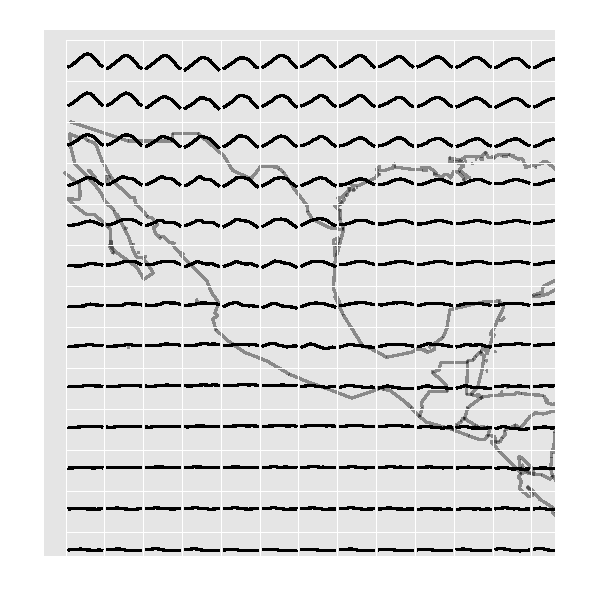
\includegraphics[width=3in]{month-cartesian}
%   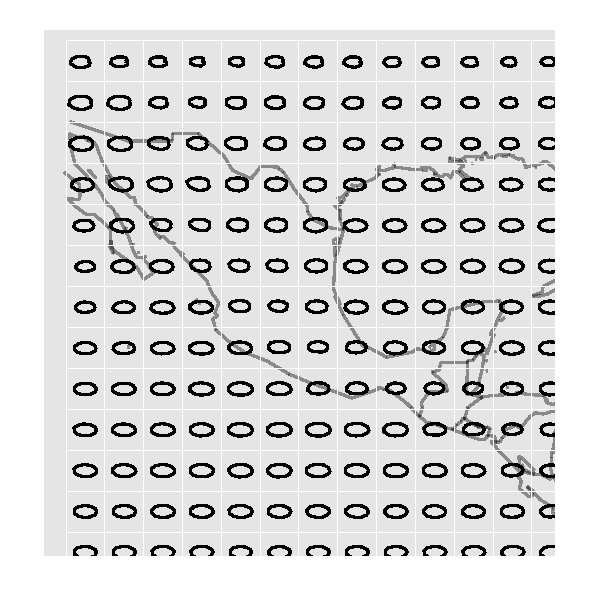
\includegraphics[width=3in]{month-polar}
%     
%   \caption{Monthly averages in (left) Cartesian coordinates and (right) polar coordinates.}
%   
%   \label{fig:cycle}
% \end{figure}

Figure~\ref{fig:templates} gives some small examples of time series with prototypical trends, shown both in cartesian coordinates and polar coordinates. Differences between linear and nonlinear trend are more apparent in the line-glyphs, and are effectively lost in the star-glyphs, which are most effective in exposing cyclical patterns due to seasonality. Star-glyphs show seasonality as floral cartoons, with peaks forming petals. It is surprising that time series with opposing trends in line-glyphs don't show this symmetry when displayed with star-glyphs. The area of star-glyphs coordinates mainly reflect the average value of a time series, while its shape shows deviations from the average.

\section{Perception}~\label{sec:perception}

All plots facilitate some comparisons and impede others. To decide if a plot if useful for a particular data analytic task, we need to check that the comparisons that we are interested in are the ones that a supported by the plot. Generally, for climate data, we are most interested in seeing changes in slope, or trend, average value, and variance. We argue that glyph-maps support these comparisons better because the comparisons are perceptually easier.

Glyph-maps allow time trends to be read directly from the plot. Values are mapped to position, one of the easiest properties to perceive \citep{cleveland:1984}. Perceiving time trends in faceted heatmaps is much more difficult: not only do you need to read value from color (a relatively difficult task), you also need to spot the difference between the different maps. This is challenging from a cognitive perspective \citep{healey:2011,busey} and comparisons can suffer from \emph{change blindness}, often leading to silent failure. 

This is particularly obvious when comparing Figure~\ref{fig:nasa-facet} to Figure~\ref{fig:nasa-glyph}.

% Laying time series out on the spatial grid, the main task expected of the viewer is comparing the temporal patterns from one location to the next. In contrast, in the small multiples used in the facetted colored map, the viewer is expected to compare the patterns in the maps from one year to the next, for corresponding months. (See \citet{carr:1999} for a discussion on perceptual grouping.) That is, compare and contrast maps with facetted colored map, or compare and contrast time series using the glyph-map. 

One draw-back of the glyph-maps, particularly if linear trend is displayed as an icon, is they may suffer from the Z\"ollner Illusion \citep{Zollner}, which makes straight lines look crooked, and is visible in Figure \ref{fig:gistemp-pred}.

An third alternative is to calculate the relevant statistic for each location and display these values as single heatmap. For example, to study long-term trends, we could calculate the slope of a linear model at each location and color tiles across the map by the value of the slope. The disadvantage of this approach is that it is not exploratory, and requires that we have a very precise definition of the measurement we are interested in, and it still suffers from the relative difficultly of colour perception.

Two other factors are critical for accurate perception of change: reference frames and scaling. These are described in the following two sections.

\subsection{Reference frames}~\label{sec:reference}

The structured spatial arrangement of icons in a glyph-map helps to compare the patterns of shape, like slope, intercept, or size, across icons. However, additional clues can make comparisons easier, converting the perceptual task from comparing length to the easier position along a common scale \citep{cleveland:1984}. This is also called a \emph{visual reference grid} \citep{cleveland:1993a}.

Each glyph is small, so there is not enough space for a full set of axes. Instead, we add reference lines and boxes. These need to be minimally perceptible, post-attentive \citep{healey} and de-emphasized, so as not to detract from the raw data. The \textbf{reference grid} is a box, framing each icon, which represents the spatial grid. The \textbf{reference line} is a horizontal line at mid-range. Both help to read differences in slope and intercept. Slope is read by comparing the position of left and right endpoints on the frame, or by reading the angle between the data line and the reference line. Intercept is read from ``average'' position of the line in the box: is it near the top, or near the bottom? Figure~\ref{fig:ref-basic} demonstrates both guides. We draw them in white, so they are minimally perceptible relative to the black data.

% , making it easier to compare the slopprovides for better reading of the intercept. The average value for the temperature anomaly data is not the same across the map: at higher latitudes the temperatures are uniformly higher, but at lower latitudes they are uniformly lower. (**** Can this be right? Would it mean that at these locations the temperatures 1950-2010 are much higher than the reference year temperatures?)

% *** Re-do these figures with zooms in on the GISTEMP data

\begin{figure}[htbp]
  \centering
  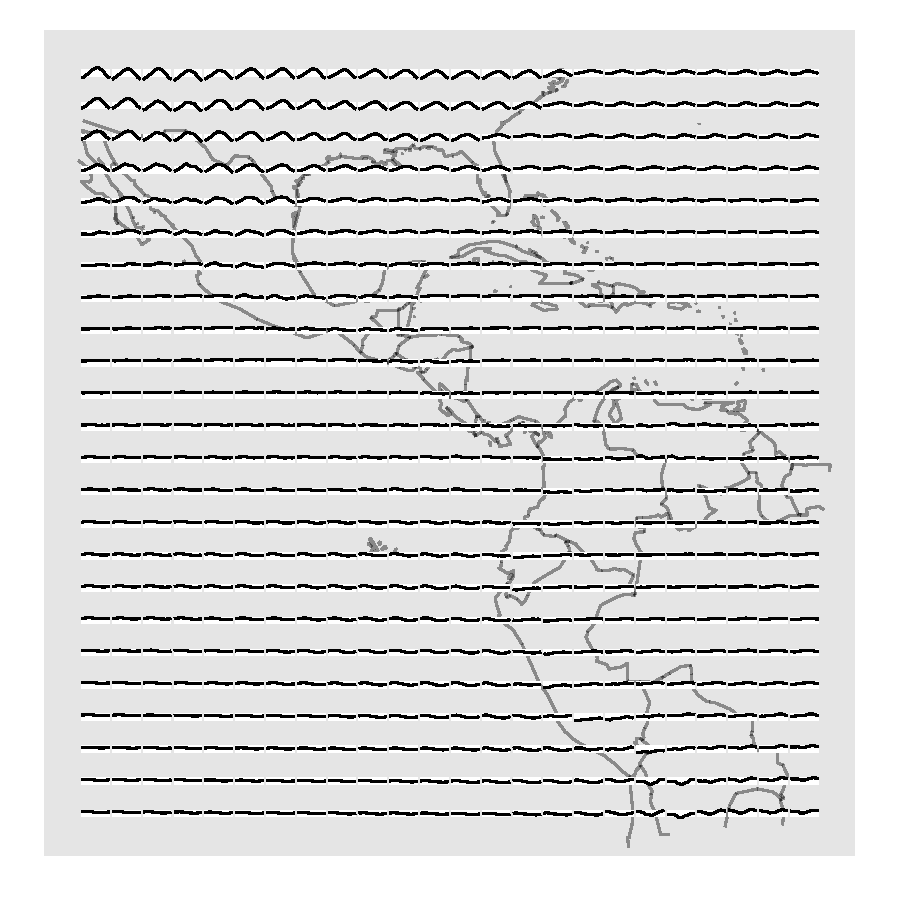
\includegraphics[width=0.5\linewidth]{ref-line}%
  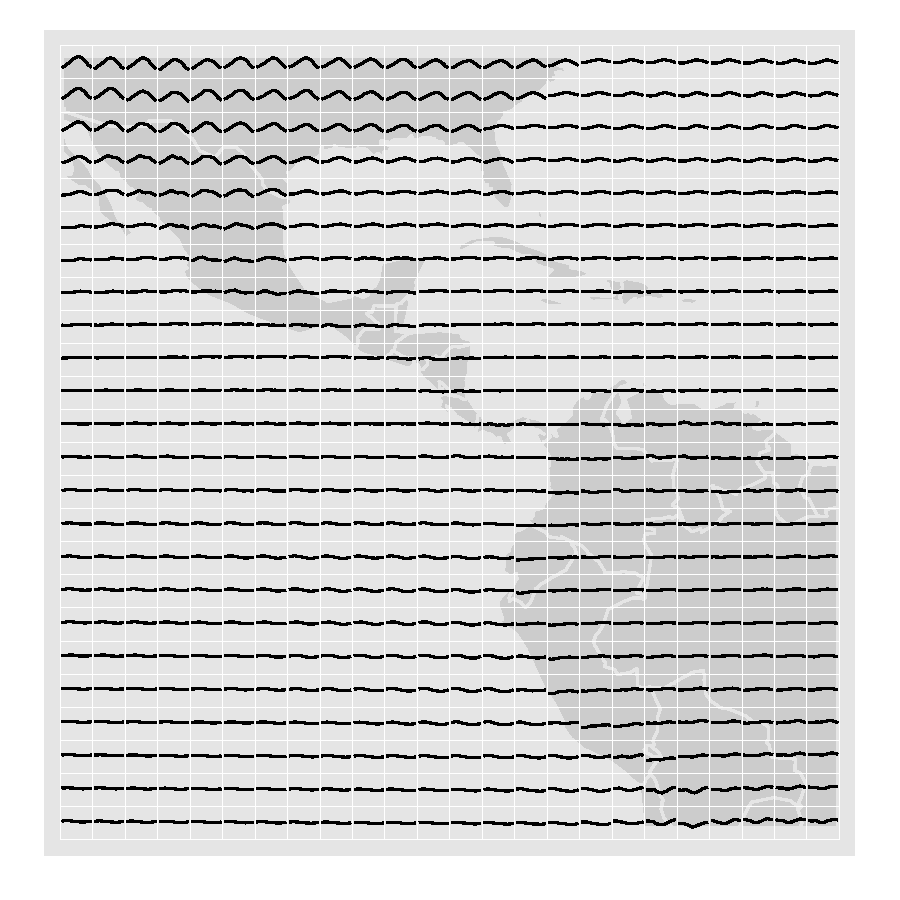
\includegraphics[width=0.5\linewidth]{ref-box}

  \caption{Glyph-maps of seasonal temperature patterns (averages for each month), using the data-expo data. Adding mid-range reference lines (left) and grid-cell reference boxes (right), makes it easier to see differences in glyph position, not just shape.}
  \label{fig:ref-basic}
\end{figure}

For star glyphs the reference frames are also useful and the equivalent of the reference line is a circle. Figures~\ref{fig:templates} and \ref{fig:gistemp-raw} show examples.

%*** Re-visit this next paragraph - its a little too airy-fairy, and the plot with color needs to have the color dampened more. Its way too dominant. This paragraph is too speculative for the paper, so removing it from first draft.

%It's also often useful to display other types of reference information. You are only limited by your imagination (and the capabilities of your graphics software), but two simple ideas are to (1) vary the colour or transparency of glyphs or references, or (2) use an additional layer to highlight special points. Figure~\ref{fig:ref-adv} illustrates these ideas to display the month with the highest temperature at each locations. Careful colour choice is necessary so that this information is perceptible, but not distracting.

%\begin{figure}[htbp]
%  \centering
%  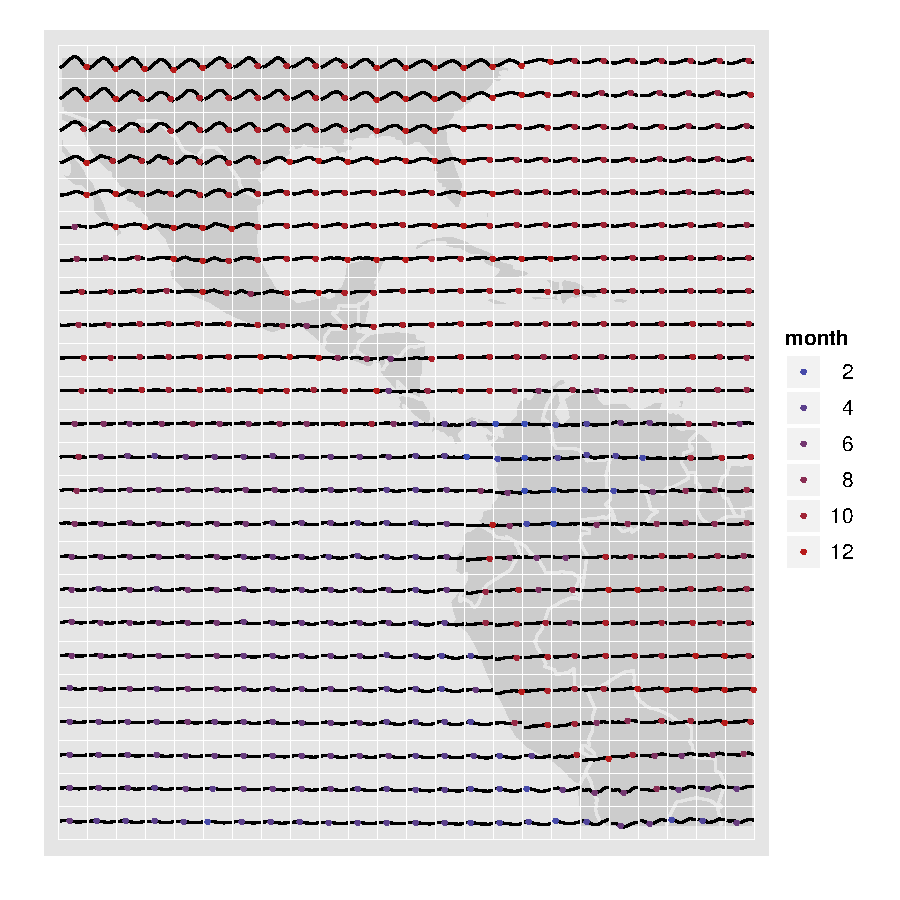
\includegraphics[width=0.5\linewidth]{ref-max-1}%
%  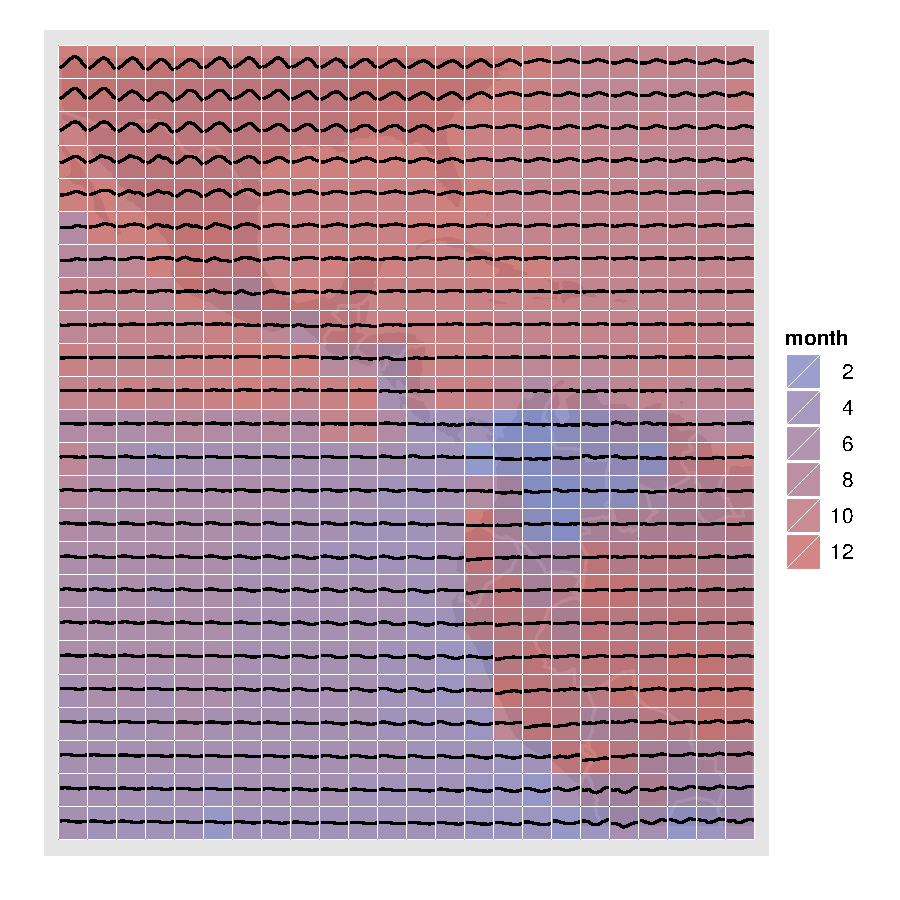
\includegraphics[width=0.5\linewidth]{ref-max-2}
%  \caption{Glyph-maps of seasonal temperature patterns also showing the month with the highest temperature using (left) an additional layer of points and (right) changing the background colour of the reference grid.}
%  \label{fig:ref-adv}
%\end{figure}

%A particularly useful summary when to add when displaying model predictions, is some measure of model fit. This makes it easier to avoid over-interpreting predictions from poorly-fitting models.

\subsection{Scaling}~\label{sec:scale}

%*** This section needs to have plots re-done, once we have decided on the key pieces

We can also emphasize different features of the data by varying the scale used with each cell. By default, we use a global scale, so the same position within each cell corresponds to the same value in all locations. This facilitates the comparison of absolute values, and draws attention to plots with large overall variation.

Alternatively, we can re-scale values within each location prior to plotting. In local scaling, the values within each location are scaled to range $[0, 1]$ before plot construction. This makes it easier to compare shape (ignoring amplitude), and draws attention to locations with large relative variation. Figure~\ref{fig:scaling} compares global scaling and local scaling for the smoothed temperature data from the data-expo data. On the global scale, the El Ni\~no blip in temperature is just visible, along with variation in the average temperature at each location. Local scaling emphasizes the individual shapes: we see the impact of El Ni\~no over a wider region, dramatic linear increases across the Andes, and decreases in the Gulf of Mexico.

\begin{figure}[htbp]
  \centering
  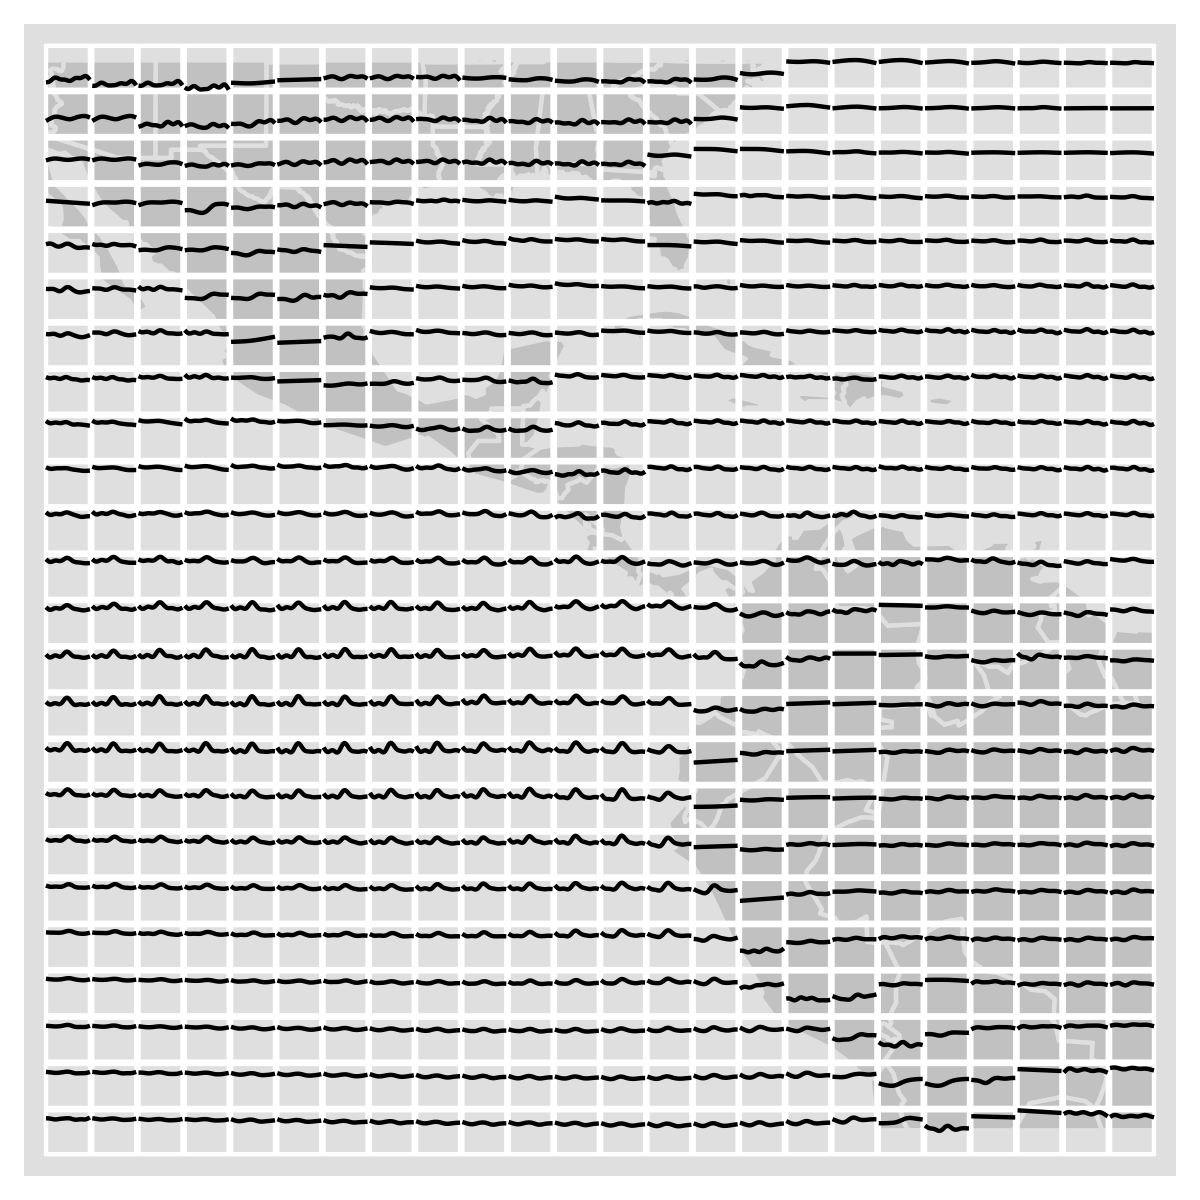
\includegraphics[width=0.5\linewidth]{month-rescale-none}%
  % 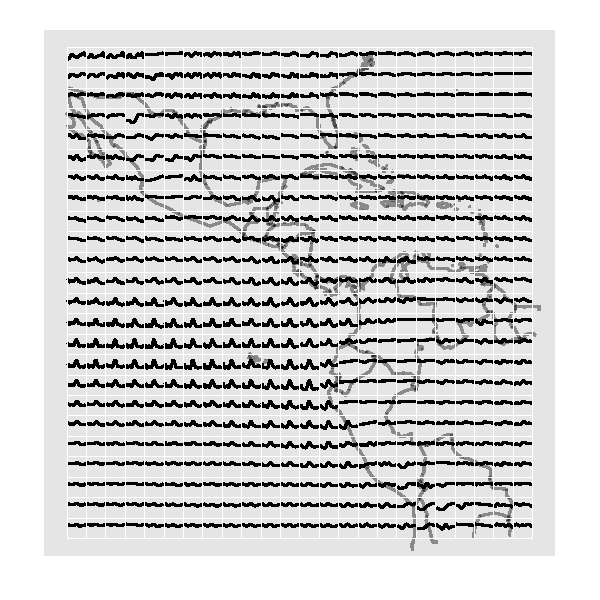
\includegraphics[width=0.5\linewidth]{month-rescale-max}%
  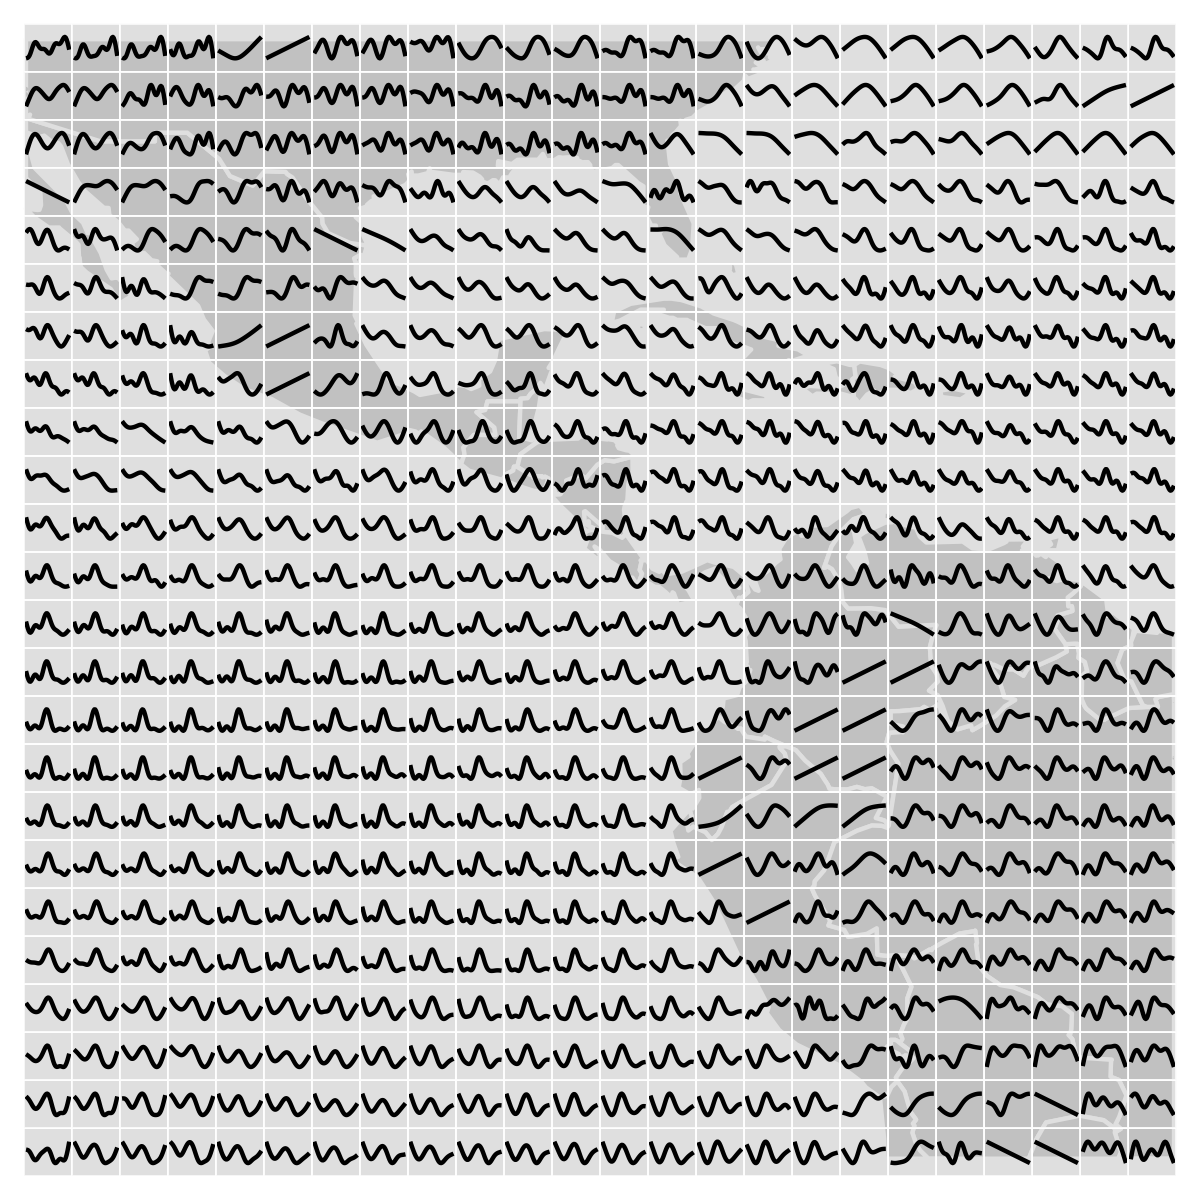
\includegraphics[width=0.5\linewidth]{month-rescale01}
  \caption{Smoothed de-seasonalized daily temperature glyph-map. (Left)
globally scaled, (right) locally scaled.}
  \label{fig:scaling}
\end{figure}

% 
% \begin{equation}
% y_{st} = \frac{y_{st}-y_{min}}{y_{max}-y_{min}} %\times 2 - 1
% \label{scale1}
% \end{equation}
% 
% \noindent where $y$ is the variable used on the minor axis in equations \ref{coords.eqn}, \ref{coords.polar.eqn}, $y_{min} = \mbox{minimum}\{y_{st}; s=1, \dots S, t=1, ..., T \}, y_{max} = \mbox{maximum}\{y_{st}; s=1, \dots S, t=1, ..., T\}$, $S=$ is the number of spatial locations and $T=$ is the number of time points. In addition, $y_{st}$ may be further scaled by doubling and subtracting 1 to give values between -0.5 and 0.5 for using in equations \ref{coords.eqn}, \ref{coords.polar.eqn}.
% 
% \begin{equation}
% y_{st} = \frac{y_{st}-y_{s,min}}{y_{s,max}-y_{s,min}} %\times 2 - 1
% \label{scale2}
% \end{equation}
% 
% \noindent where $y_{s, min} = \mbox{minimum}\{y_{st}; t=1, ..., T \}, y_{s,max} = \mbox{maximum}\{y_{st}; t=1, ..., T\}$. 

Other types of shifting and scaling can be useful:

\begin{itemize}

  \item The mean and standard deviation (or robust equivalents) could be used
  to standardize values to common moments.
  
   \item Scaling to maximum 1 (but leaving the minimum unchanged) can help
  emphasis the relative shape, but not distort the range as much as rescaling
  to range $[0, 1]$.

  \item Shifting the values at each location to have mean zero places more
  focus on the trend. This is particularly important for the star glyphs,
  where differences in the average value lead to unintuitive patterns in the
  resulting glyphs.

\end{itemize}

Note that the use of local scales needs to be clearly marked. The viewer must realize that the scale is not relative and that big patterns in some locations might be just tiny effects. To indicate this on the locally scaled data plots, one can use an additional aesthetic, like colour, to encode the original scale.  This is illustrated in Figure~\ref{fig:scaling-col}.

\begin{figure}[htbp]
 \centering
 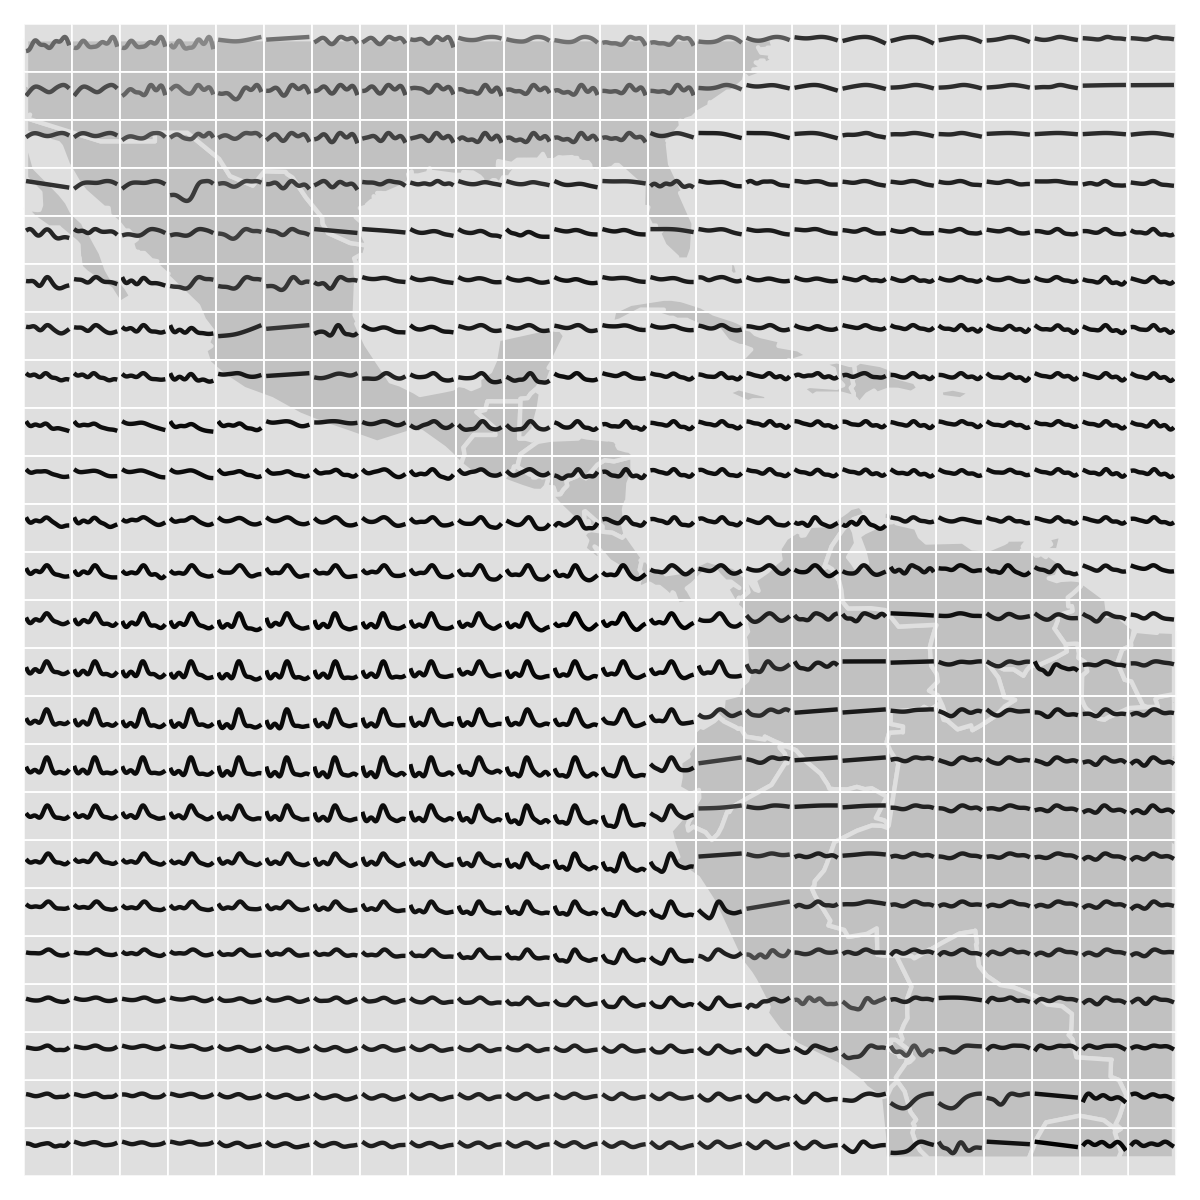
\includegraphics[width=0.5\linewidth]{month-rescale01-col}%
 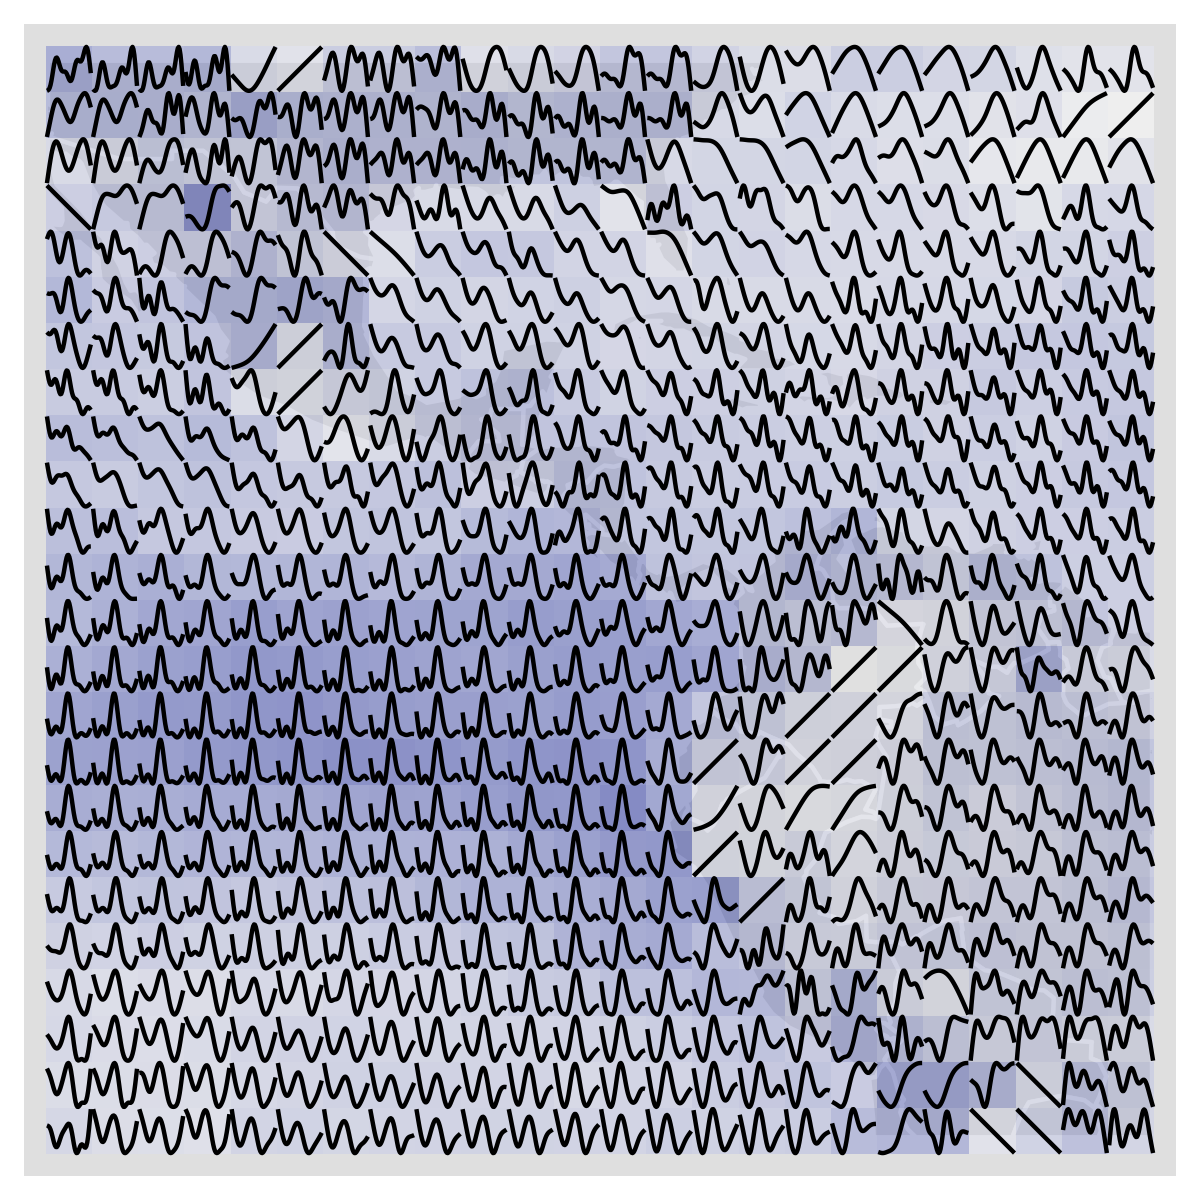
\includegraphics[width=0.5\linewidth]{month-rescale01-fill}
 \caption{Adding colour to scaled plots. Here each location has been scaled to range $[0, 1]$ and colour mapped to the range of the original predictions. Pale locations have smaller range than darker locations. Shapes at all locations are visible, but attention is drawn to locations with larger ranges.}
 \label{fig:scaling-col}
\end{figure}

One more important point: if a model summary is displayed in the glyph-map, as discussed in the following section, it may be important to force the scale to that of the original data. The range of predicted values is typically smaller than the raw data, so angles of slopes is increase.  

% Displaying the predicted values in the absence of the raw data scale typically increases magnitude because the variation is much lower.

\section{Large data and models}
\label{sec:large-data}

Climate data is usually large: many locations in space, and many points in time. This makes climate data challenging to work with computationally and to visualize. Plotting the raw data often reveals little more than a well-known observation that ``temperature is quite varied!'' Careful use of models to decompose data into long-term trend, seasonal effects and error is vital for to make the problem both computationally and visually tractable.

Figure~\ref{fig:gistemp-pred} shows the a glyph-map for the large GISTEMP dataset. Glyphs at each location represent temperature from 1880--2011, starting with Jan 1880 at 12 o'clock and proceeding clockwise to 2011 at 11:59. The most important feature to notice is the pattern of missing values. Most glyphs do not complete the full circle, typically missing points between 12 and 1, suggesting missing values in the earliest part of the data. Another important feature is variability, shown by the thickness of the circle. Some locations, particularly in the north western mountain region, have large variations in temperature. 

\begin{figure}[htbp]
  \centering
  %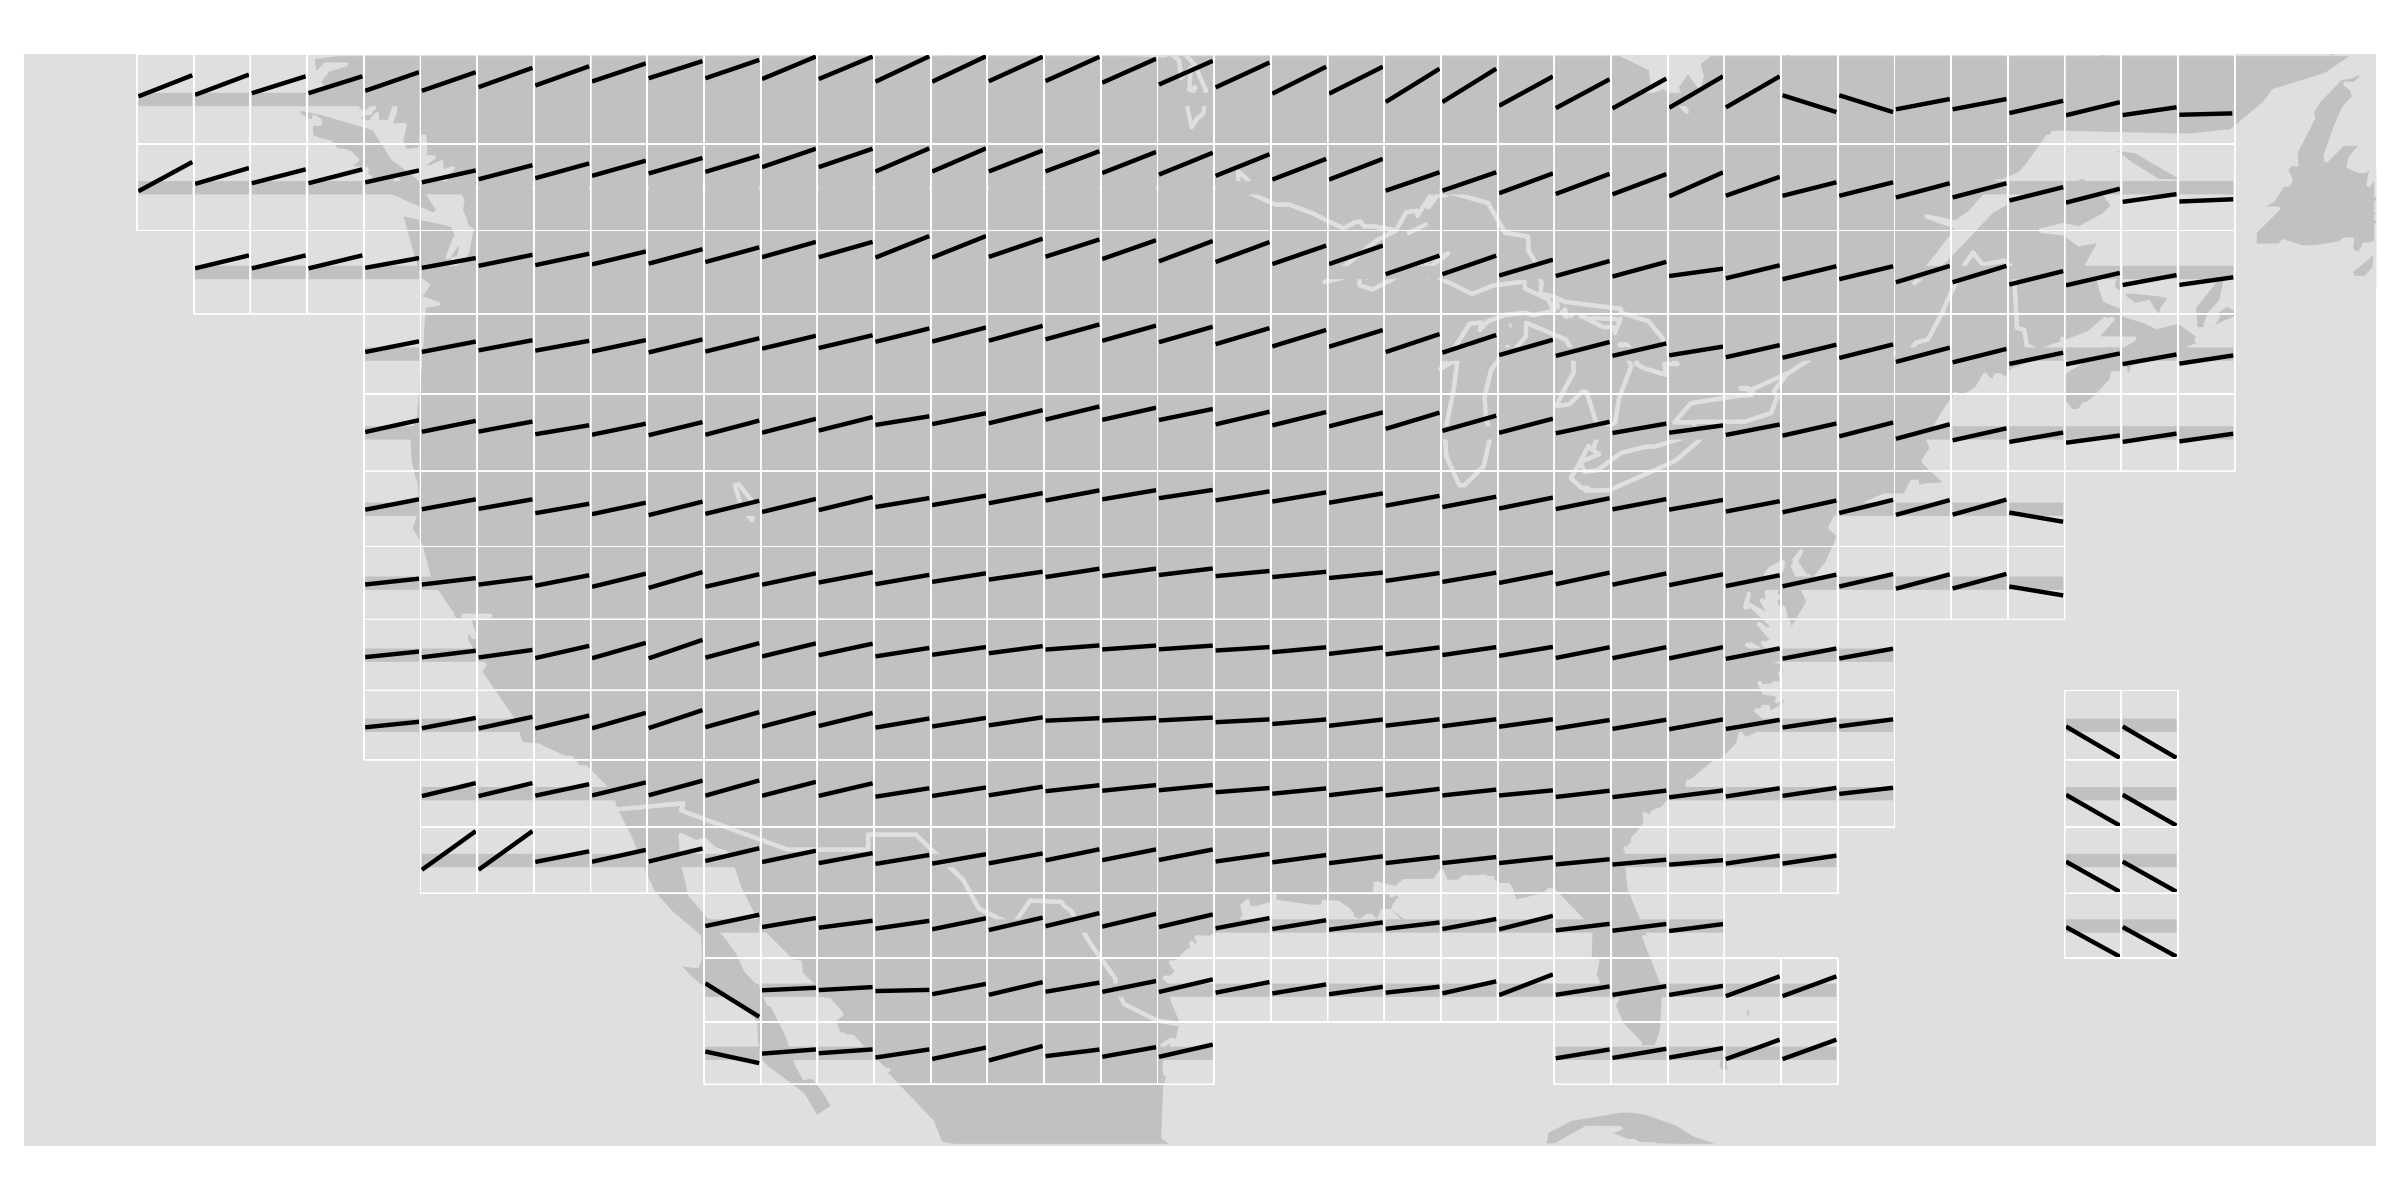
\includegraphics[width=1\linewidth]{gistemp-pred}%

  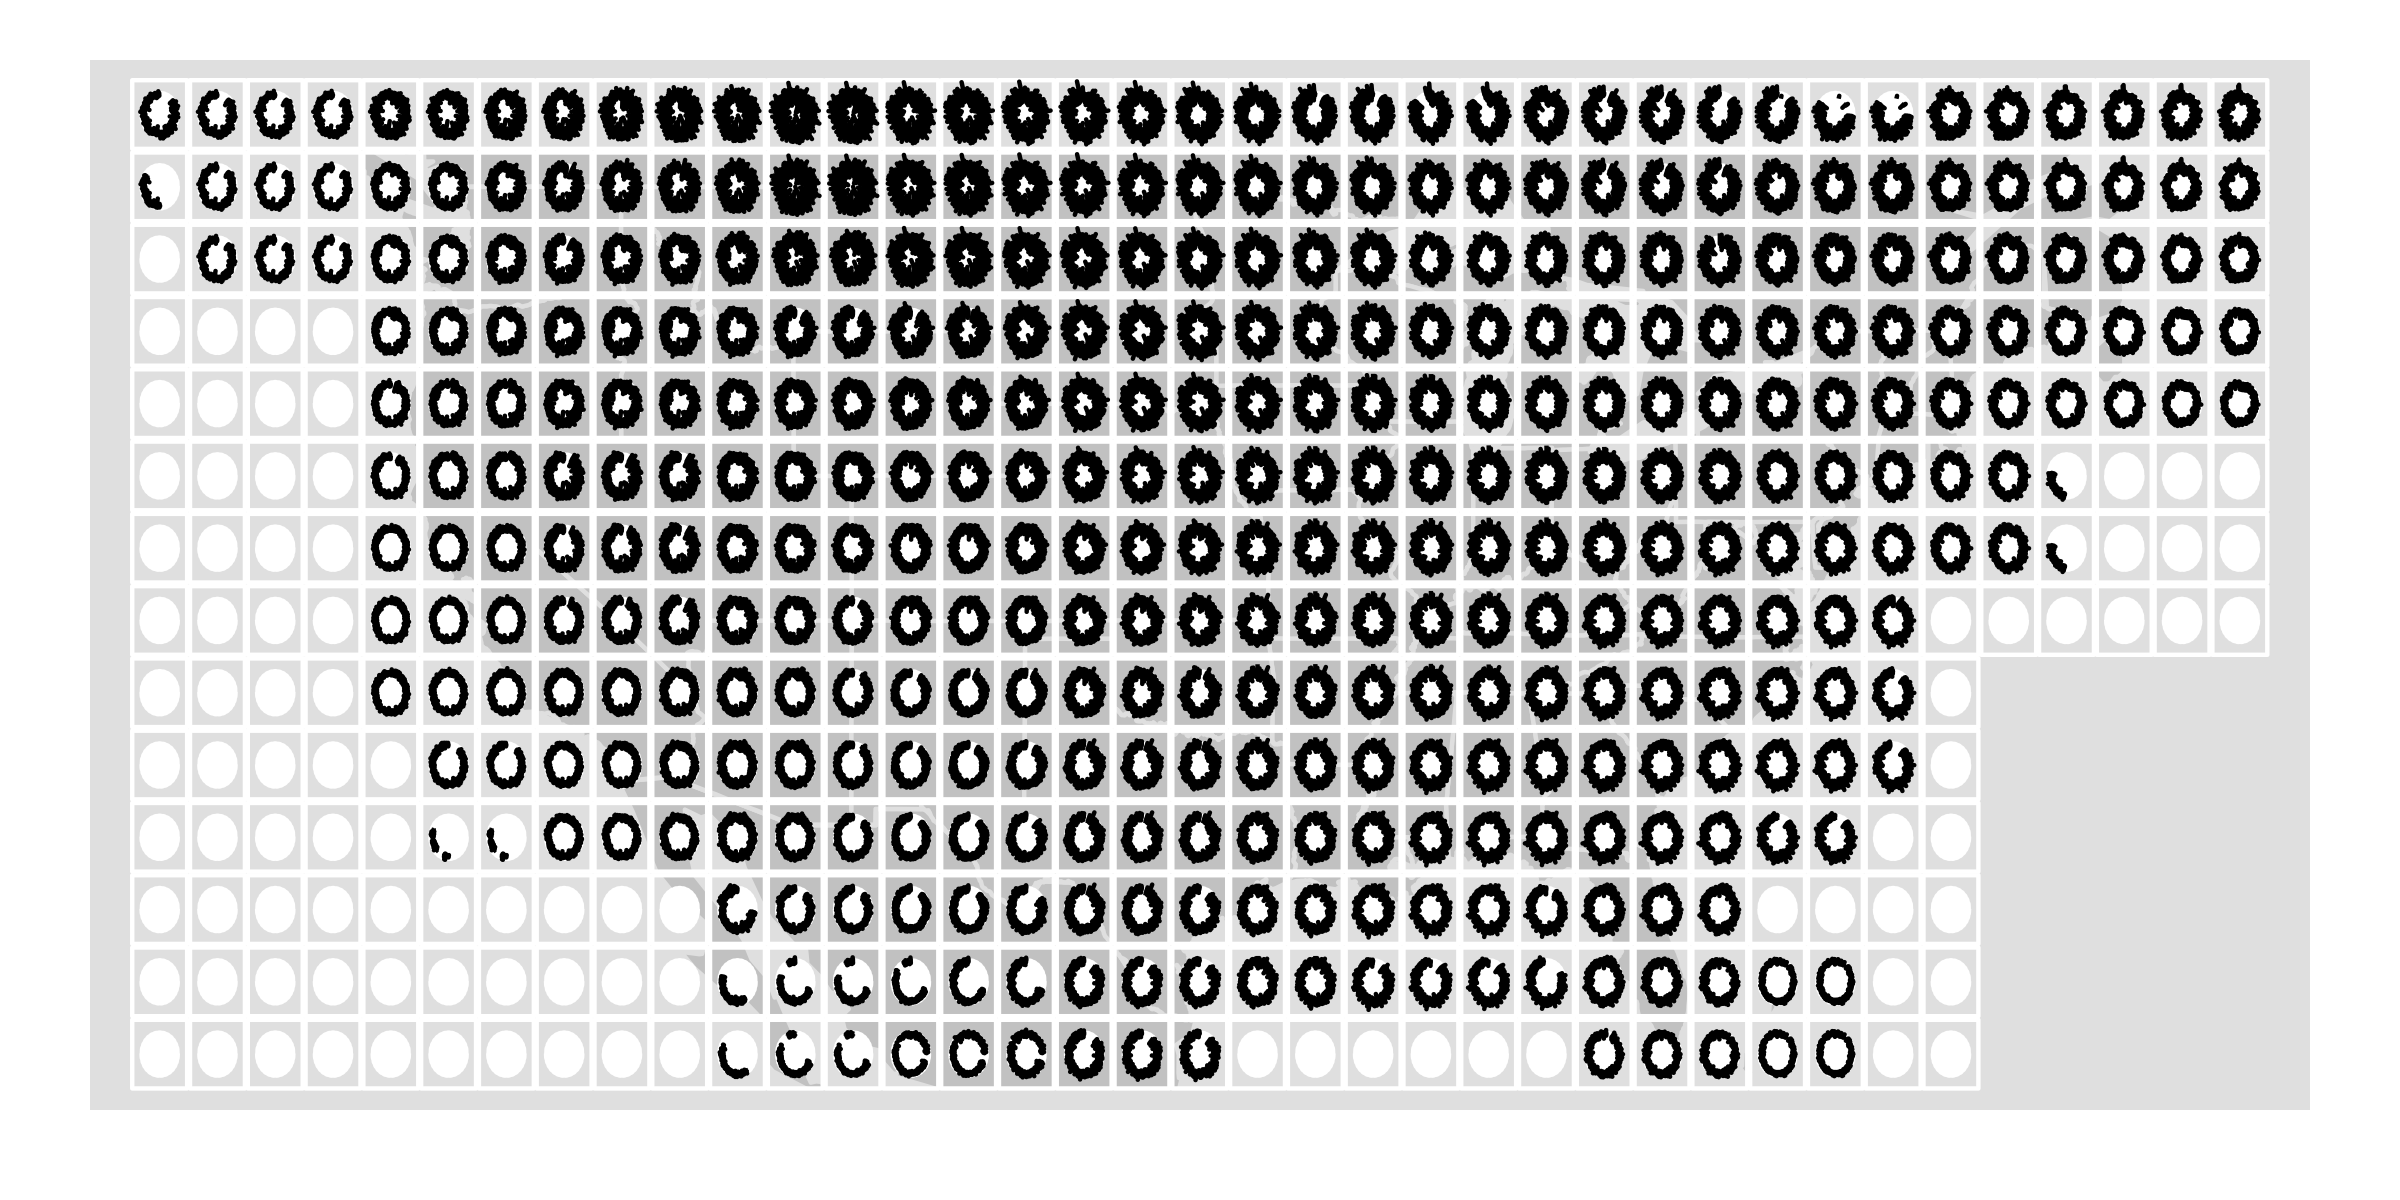
\includegraphics[width=1\linewidth]{gistemp-polar-raw}

  \caption{Glyph-map of raw temperature anomaly data, from 1880-2011. Gaps in the full circle indicate missing values, and thickness of the circle indicates more variability in the measurements.}
  \label{fig:gistemp-raw}
\end{figure}

The raw data shows us missing values and gives some sense of variability, but gives no information about long-term trend. We can look trend by fitting a linear model to each location and displaying the predicted values. Figure~\ref{fig:gistemp-pred} shows this for 1950--2010 (limited time period used due to missing data). Most locations have increasing temperature over this time period. Only a few locations show a decline. These locations tend to be different from their neighbors, which might suggest isolated data problems. The rate of increase differs across regions: steeper inclines in the north and western mountain regions and across the Great Lakes, and flatter inclines in the southeastern USA.

\begin{figure}[htbp]
  \centering
  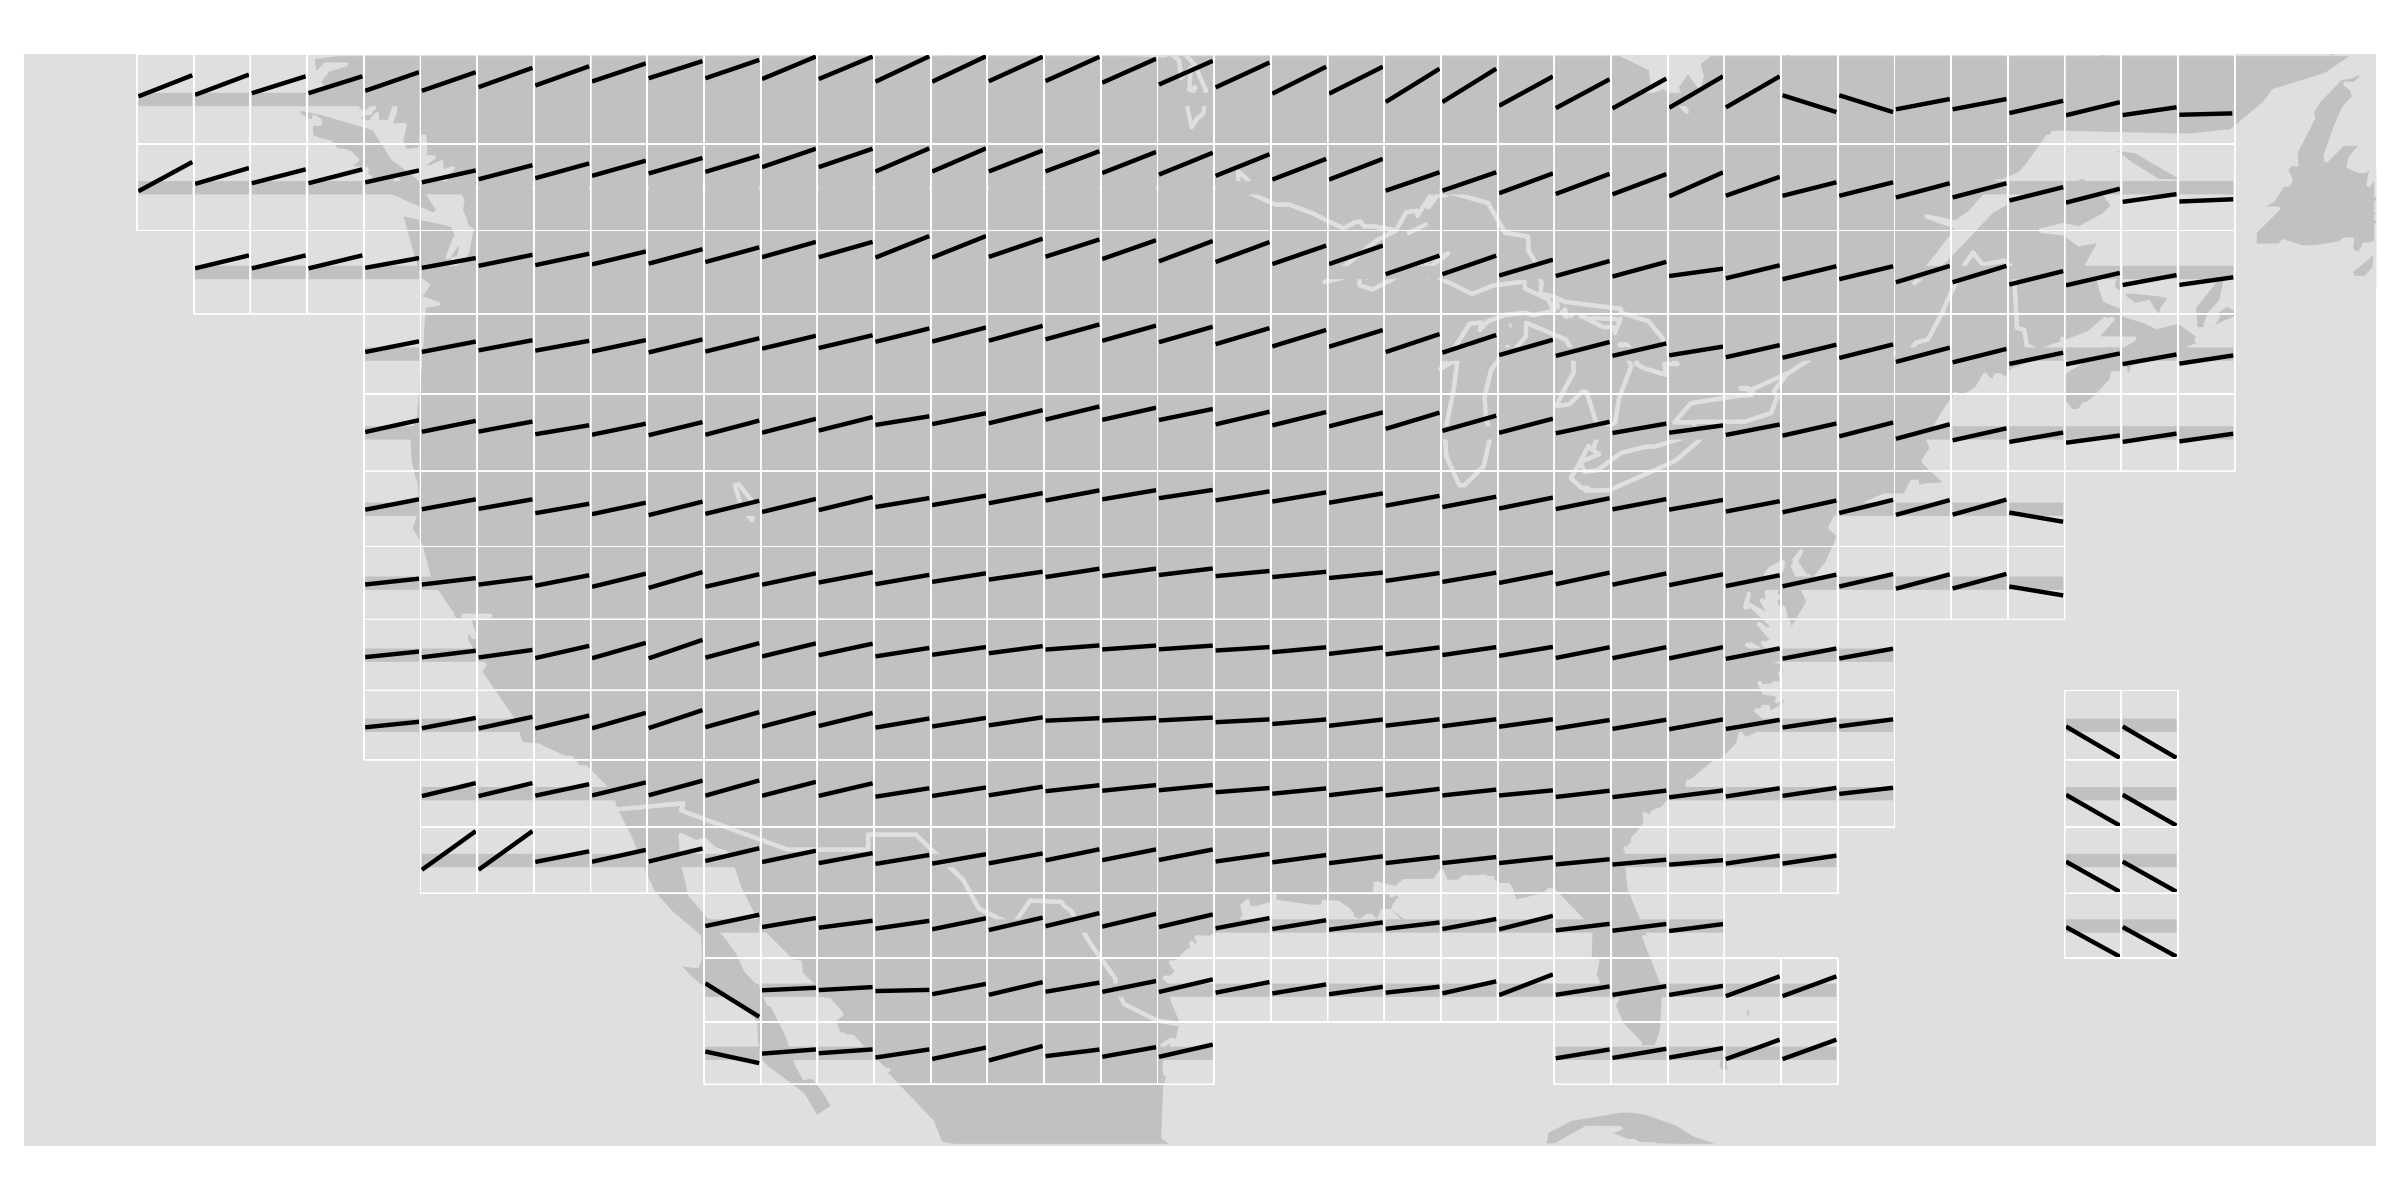
\includegraphics[width=1\linewidth]{gistemp-pred}%
  %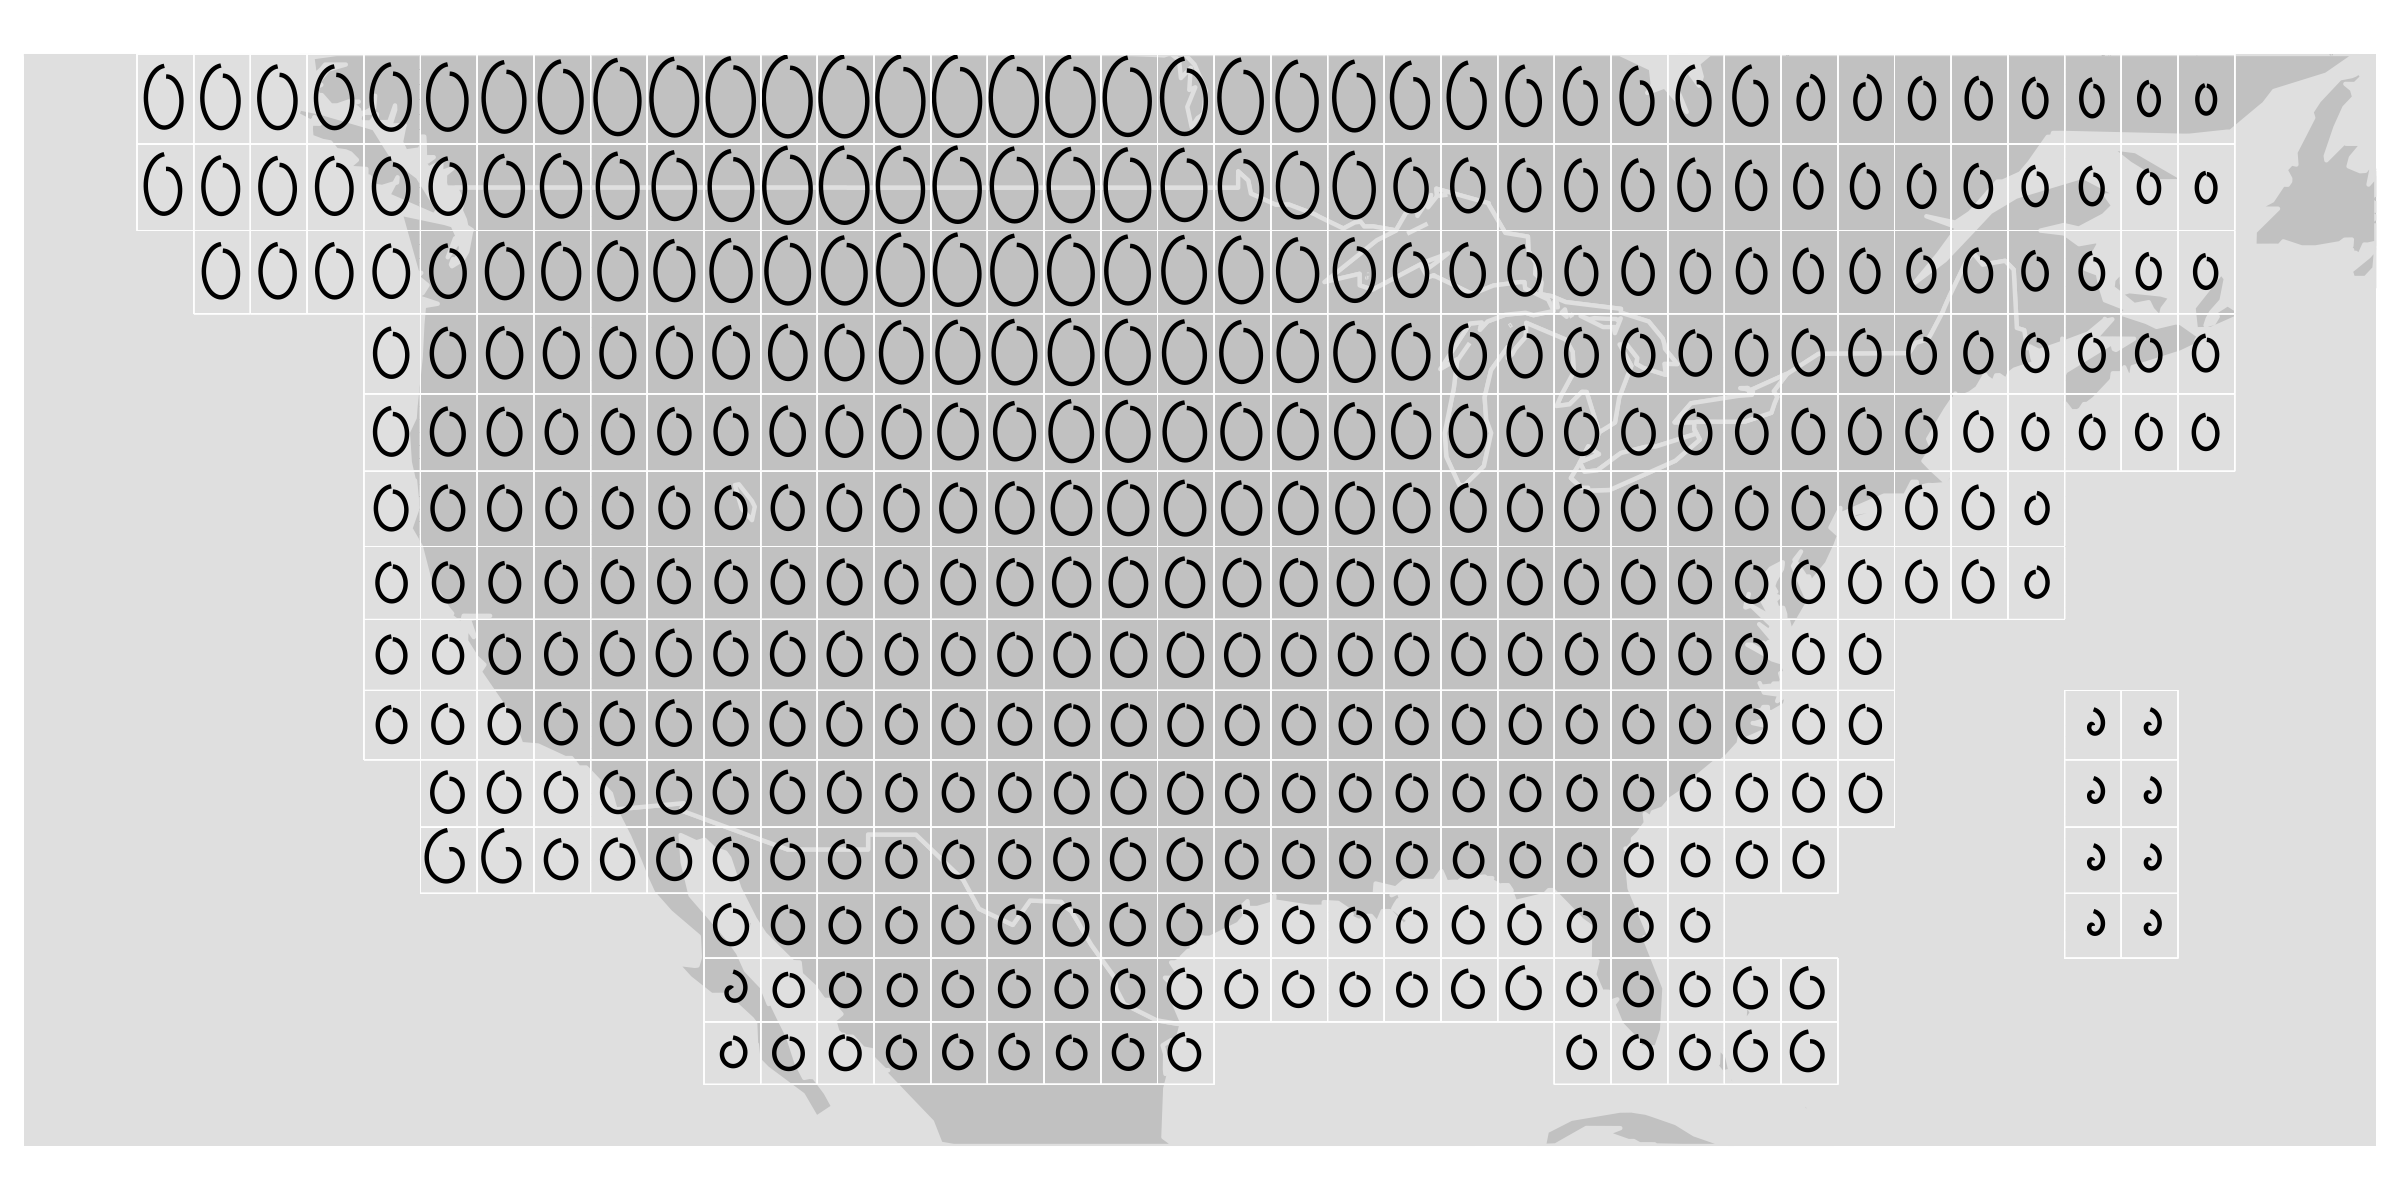
\includegraphics[width=1\linewidth]{gistemp-polar-pred}

  \caption{Glyph-map of predicted temperature anomaly data, from
    1950-2010. Increasing trends can be seen over most of the USA,
    with varying degrees of increase. Some isolated locations exhibit
    steep declines, and inclines, perhaps indicative of some isolated
    data problems.}
  \label{fig:gistemp-pred}
\end{figure}

%The most seasonality occurs in north American. Some seasonal effects can also be seen in the Caribbean and in south American locations. Around the equator the temperatures are relatively warm for all seasons. Instead of radially displaying the temperature a glyph can be a regular time series, time displayed horizontally and temperature vertically (right plot). The structure perceived is different with this change in glyph type: locations at the equator have flat series, on land more varied temperatures. 

% \section{What to plot: raw data, trend lines, residuals,  seasonal}
% 
% A generalized additive model \citep{wood:2006} with a seasonal term and a long-term smooth term can be useful. This is revealing for smooth models of surface temperature, shown in Figure~\ref{fig:scaling}. Each location is modeled using a generalized additive model \citep{wood:2006} with a seasonal term and a long-term smooth term. The three plots in the figure show the long-term smooth term. 
% 
% %Because some locations are uniformly warmer than others, the impact of
% %changes across time are diminished. In the center plot, each location is
% %scaled by dividing out the maximum, and on the right, each location is scaled
% %to range $[0, 1]$. These emphasize individual changes but lose the ability to
% %make global comparisons, and need caution when interpreting - a small
% %absolute change gets blown up into a large relative change.
% 
% *** Need three plots here: trend, seasonality and residuals, shall we do this with NASA ozone data or stick to temperature?
% 
% Issues of scale relative to modeling. Switching from the data to model summaries brings new scaling issues. Often the scale of the raw data is ignored when the model is plotted, one usually shows just the line showing the trend, in the range of the trend. This has the effect of exaggerating the significance of the model. Scaling the trend lines relative to the range of the data may be useful sometimes.

\section{Non-gridded data}~\label{sec:irregular}

Regularly gridded spatial data helps with the perception of structure, because it helps to provide the reference frames upon which to make comparisons among the icons. When spatial locations are not on a regular grid, some difficulties arise. In this situation it is not clear what the scale of icons should be, there is no regular spacing. Some locations may be close to each other which would generate icons that overlap. 

\subsection{Non-rectangular grids}

Glyph-maps work best when displayed in the coordinate system in which the grid is rectangular and regular.  For example, the GISTEMP grid is 2$^o$ square and is displayed treating longitude and latitude as cartesian coordinates in Figure \ref{fig:gistemp-pred}.  For regularly gridded data, this results in icons that are rectangles of equal size.  It is often preferable to display maps as a projection of the geographical coordinates which preserves a property of interest, area for example. When a projection is desired a choice needs to be made between applying the projection to the completed glyph-map, or to just the spatial locations.  When the completed glyph-map is projected the icons are no longer rectangles of the same size but they do retain their space filling property.  When applying a projection to the spatial locations and then constructing a glyph-map, the grid becomes irregular. 

\subsection{Irregular locations}
Figure \ref{fig:irregular} shows linear trends for monthly average surface temperature at stations in the USHCN (Version 2) ground station network.  It illustrates three challenges in working with irregular locations: there is no natural choice for icon size, icons can potentially overlap, and comparisons rely more heavily on the reference guides.  The icon sizes were chosen manually for these two plots, although the icons are displayed at about the same size, they correspond to 1$^o$ and 0.5$^o$ square respectively in the geographical coordinates. 
\begin{figure}[htbp]
  \centering
  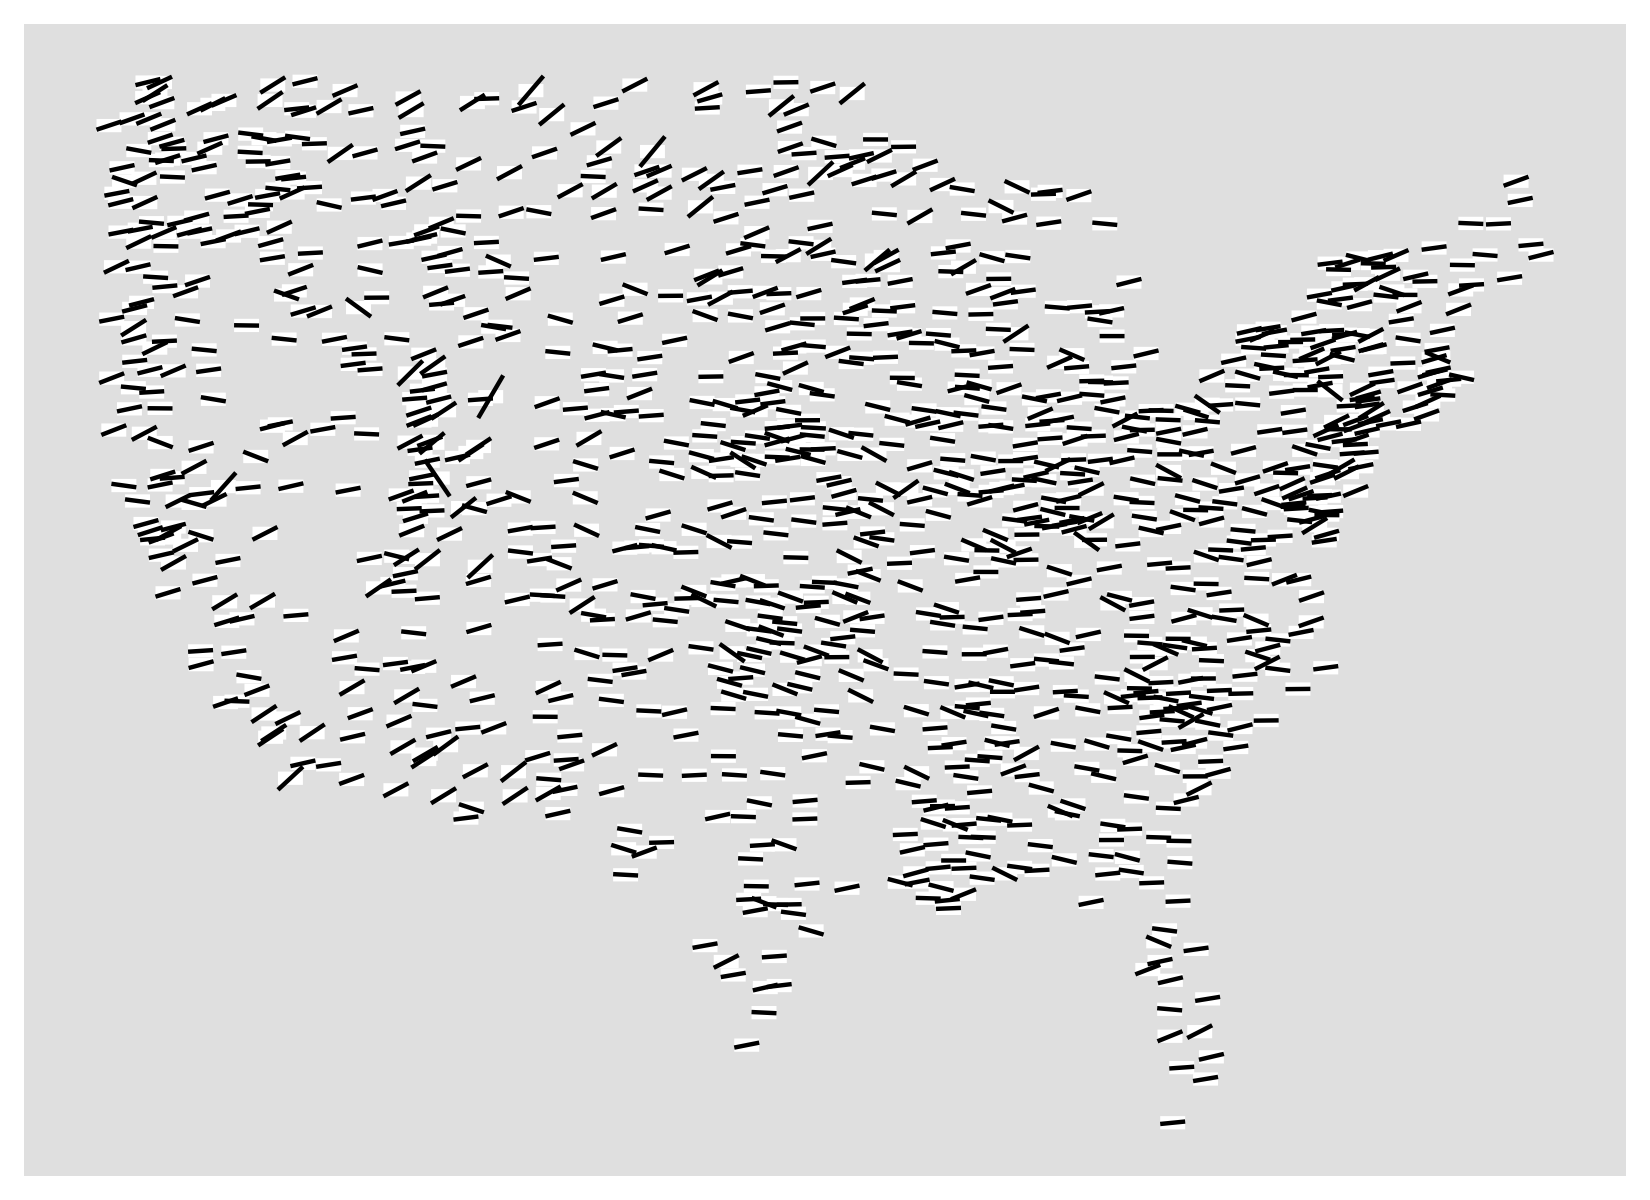
\includegraphics[width=0.55\linewidth]{usa-lin-overlap}%
  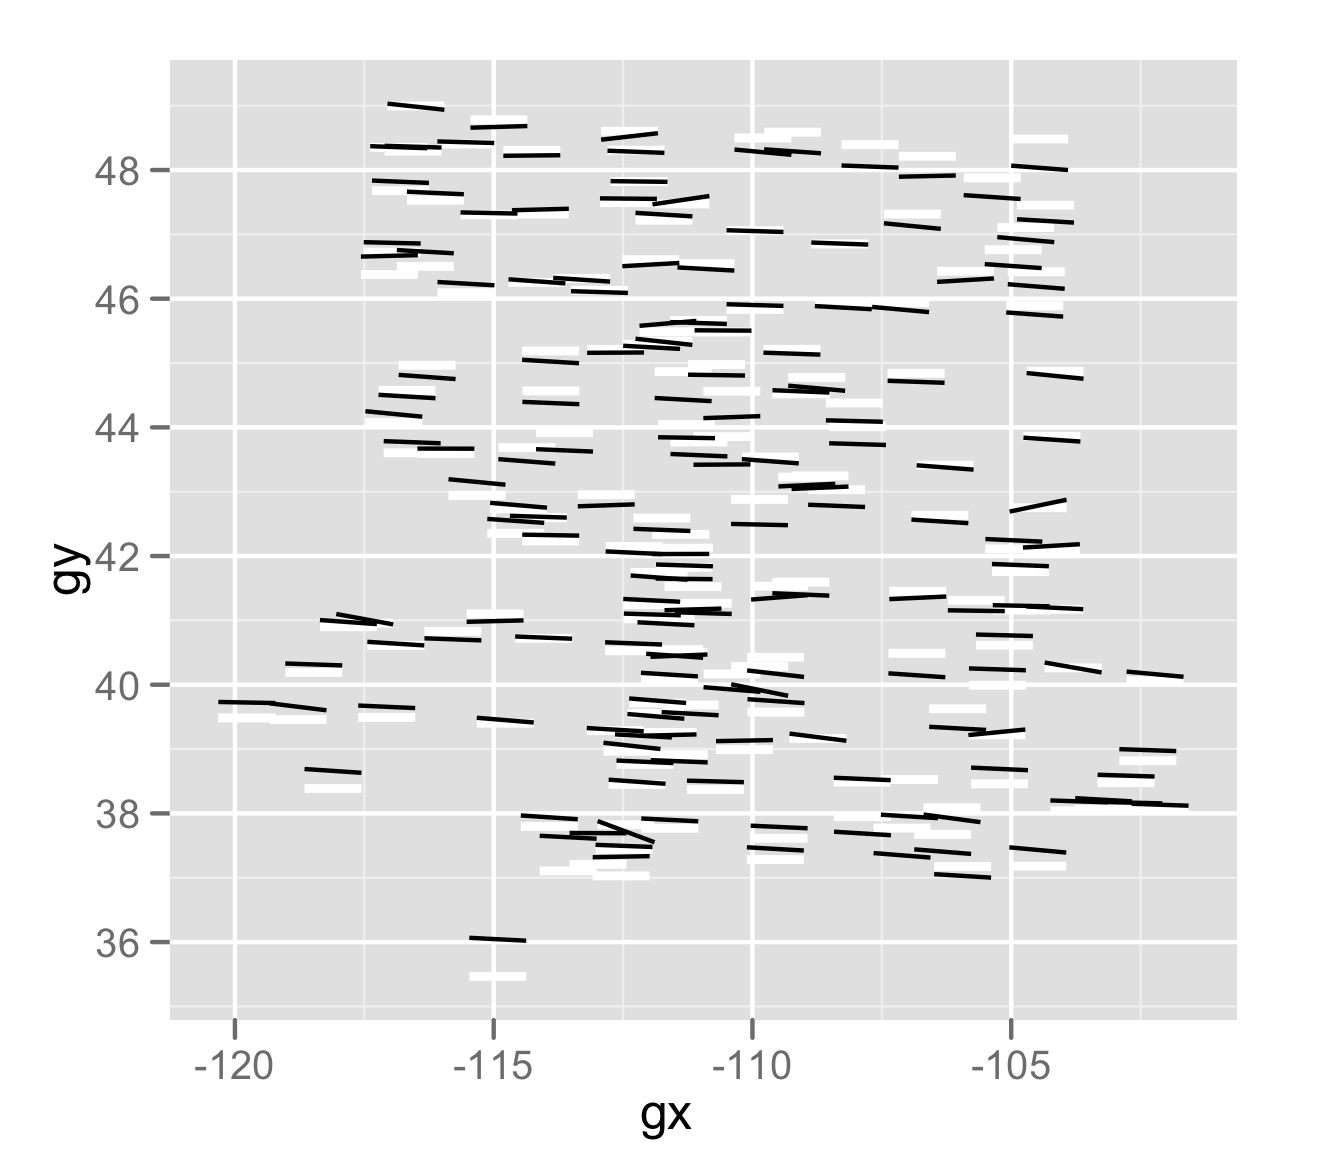
\includegraphics[width=0.35\linewidth]{ghcn-mountains}%
  \caption{Glyph-maps of the linear trend in ground station temperature values, 1950--2010, for all continental US USHCN stations (left) and stations in the mountain states (right).} 
  \label{fig:irregular}
\end{figure}
The two panels illustrate one approach to the overlapping problem: zooming.  There is an interplay between icon size (in geographical units), plotting area (in geographical units) and plot size (in display units).  Icons need to be big enough to be readable on the display, but small enough to avoid overlapping.  Readability can be maintained and overlapping reduced by decreasing the icon size and simultaneously increasing the display size or decreasing the plotting area (as done in the right panel in Figure \ref{fig:irregular}).  However, there are generally limitations in the maximum display size (or resolution) and the utility of plotting very small areas.  

An alternative approach is to combine overlapping locations and plot a single summary icon.  In Figure \ref{fig:irregular-collapsed} nearby locations are collapsed to a single icon.  In the left panel each station still has an individual glyph but locations close to each other share a plotting area.  Not all glyphs are suited to this kind of space sharing, another option is to perform a summary of the locations that are collapsed and display that instead of the raw data.  The right panel shows an example of this where the average trend for the collapsed locations is displayed.  It is helpful to differentiate glyphs that involve summaries of more than one location, here a heavier line indicates at least two locations have been averaged.

\begin{figure}[htbp]
  \centering
  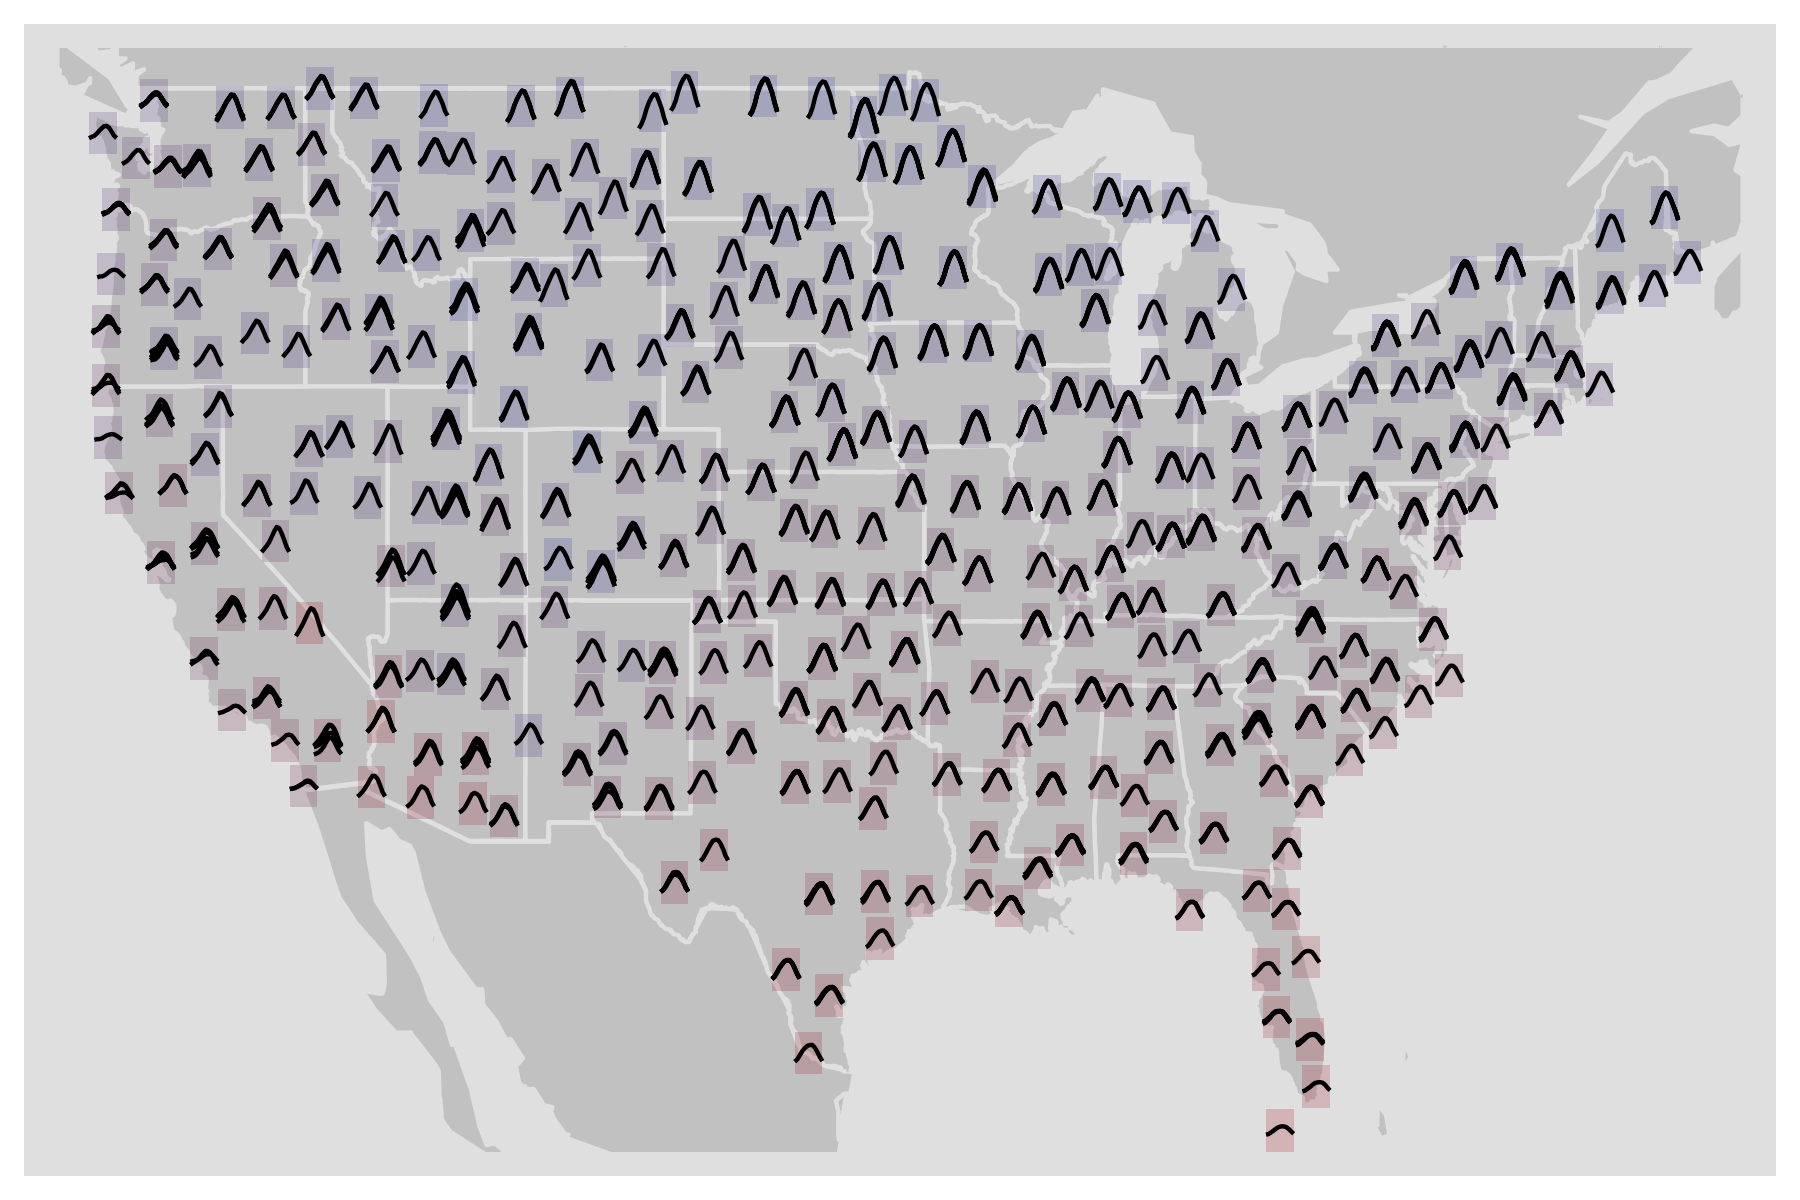
\includegraphics[width=0.5\linewidth]{usa-season-collapsed}%
  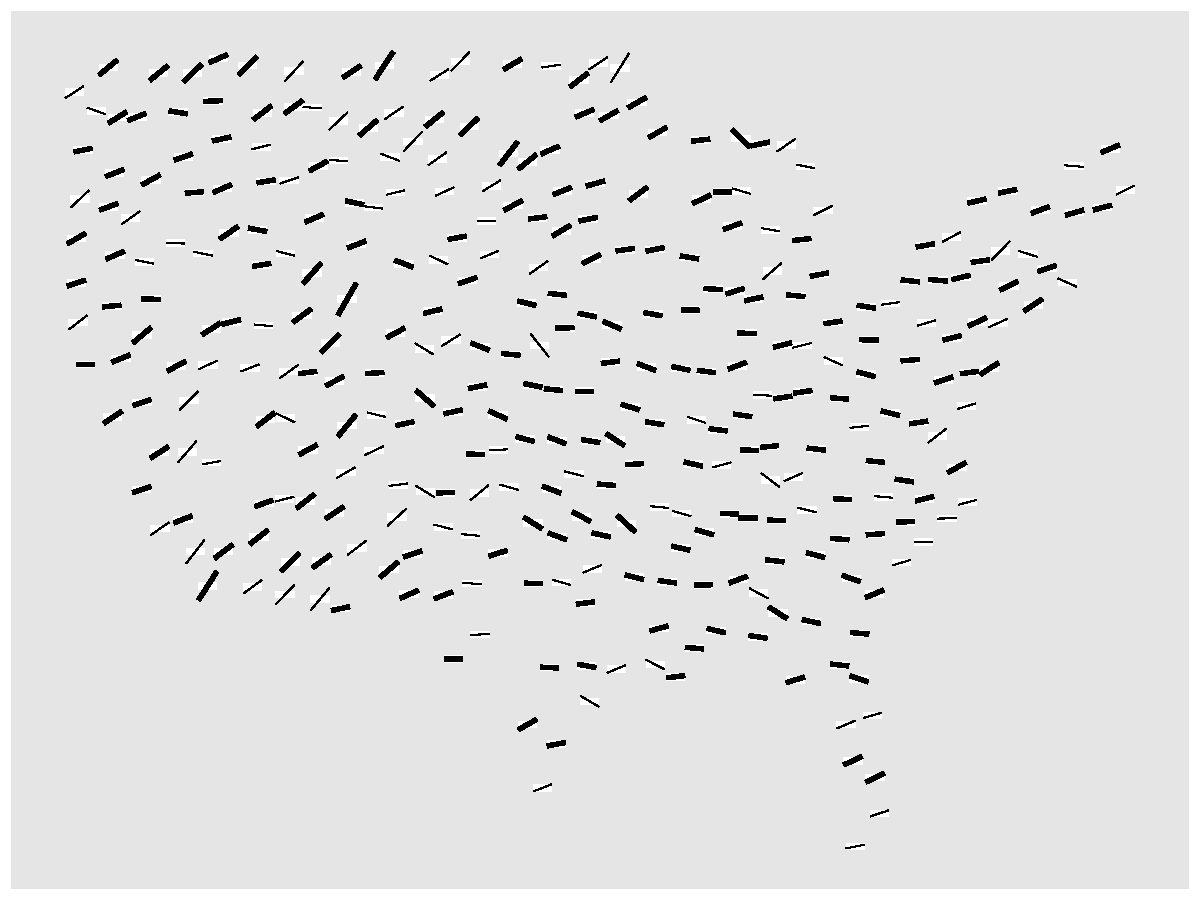
\includegraphics[width=0.5\linewidth]{usa-lin-collapse}%
  \caption{Glyph-maps of seasonal patterns (left) and linear trends (right) of USHCN stations, 1950--2010.  Nearby stations whose icons would overlap have been collapsed.  Each location has a glyph in the seasonal plot and color of the tiles corresponds to the average temperature of the locations (red=warm, blue=cool).  Heavy lines in the linear trend plot correspond to average trends over more than one location.}
  \label{fig:irregular-collapsed}
\end{figure}

In both examples of collapsing locations, the icon locations still represent real geographical locations of data, but contain data from up to an icon width away.  An alternative way to combine stations is to round locations to the icon size, Figure \ref{fig:irregular-grid}. This produces a regular grid with the advantage of easier perception of structure.  However, it hides the irregular nature of the locations and icons may end up centered over nonsense places (i.e. land measurements in the ocean).

\begin{figure}[htbp]
  \centering
  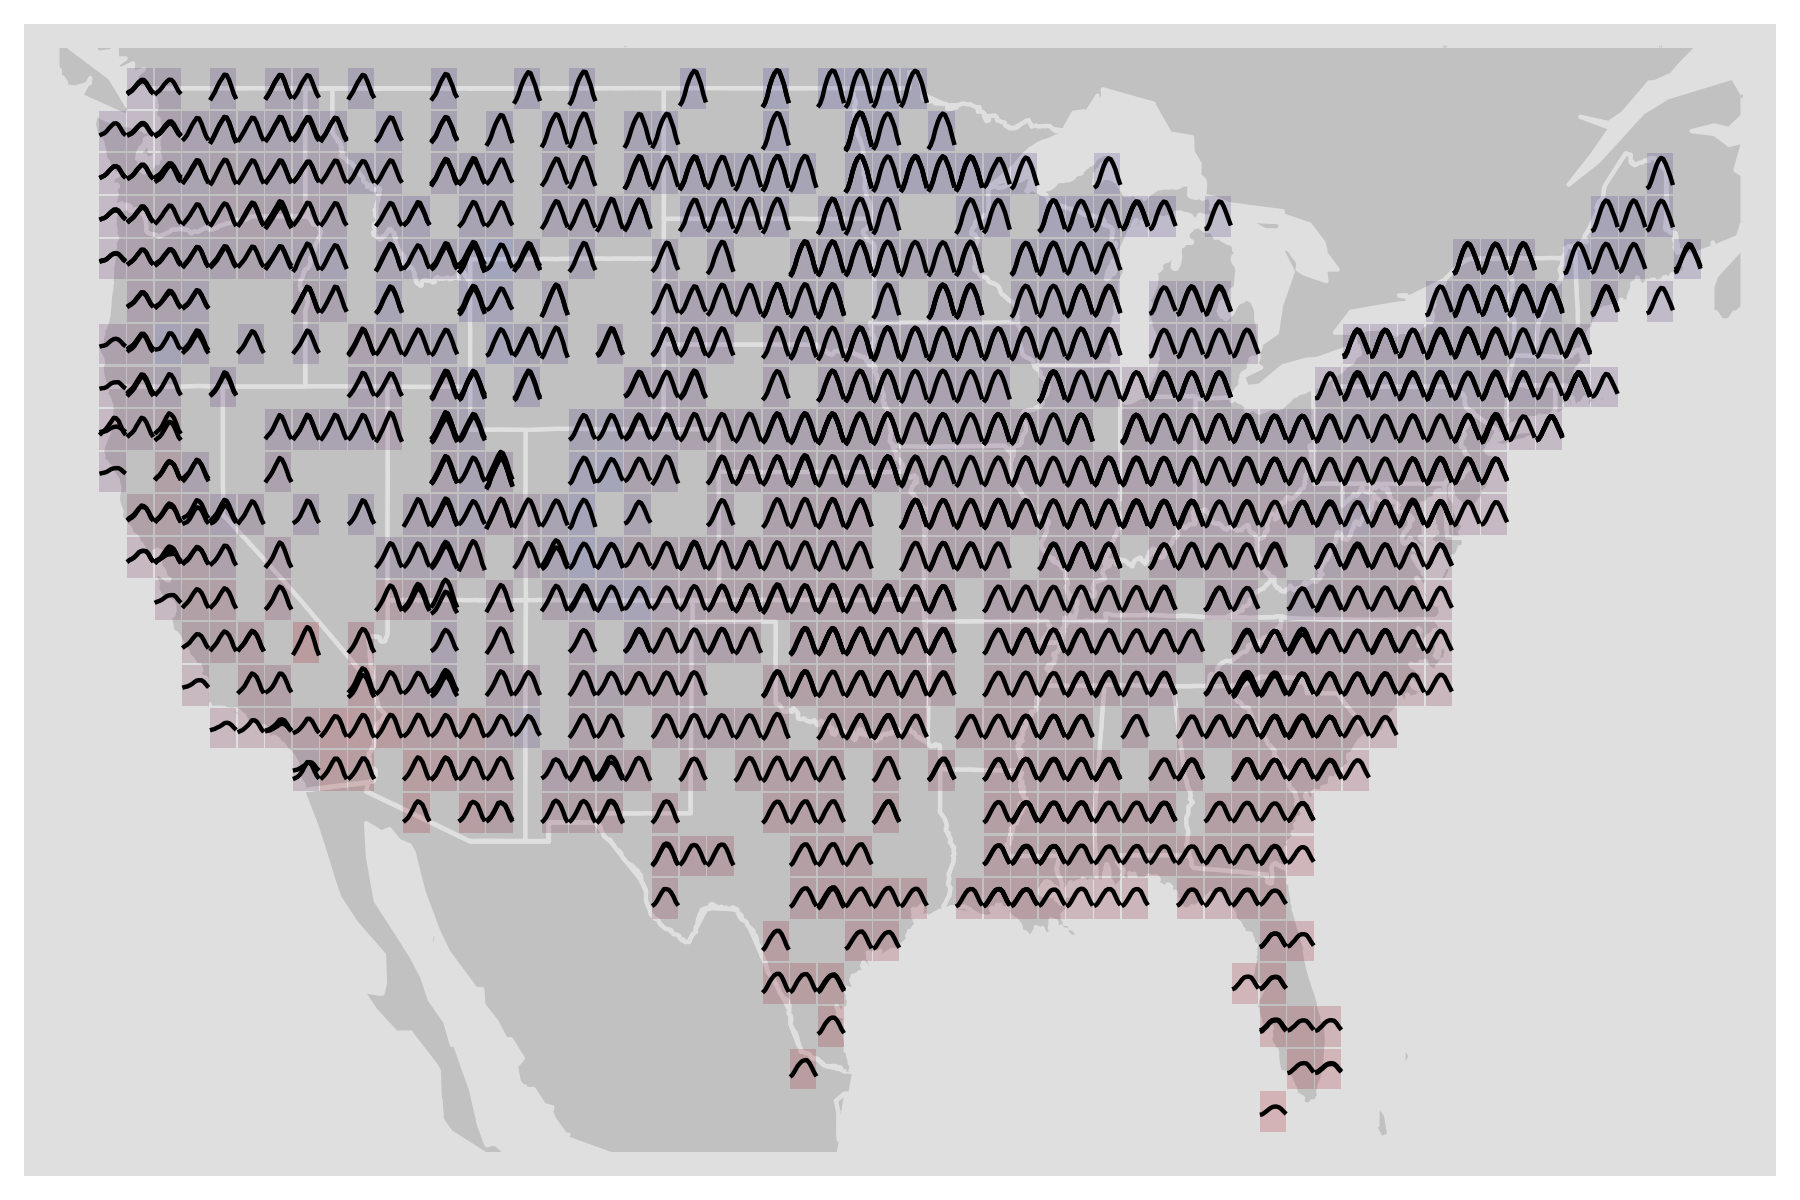
\includegraphics[width=0.5\linewidth]{usa-season-grid}%
  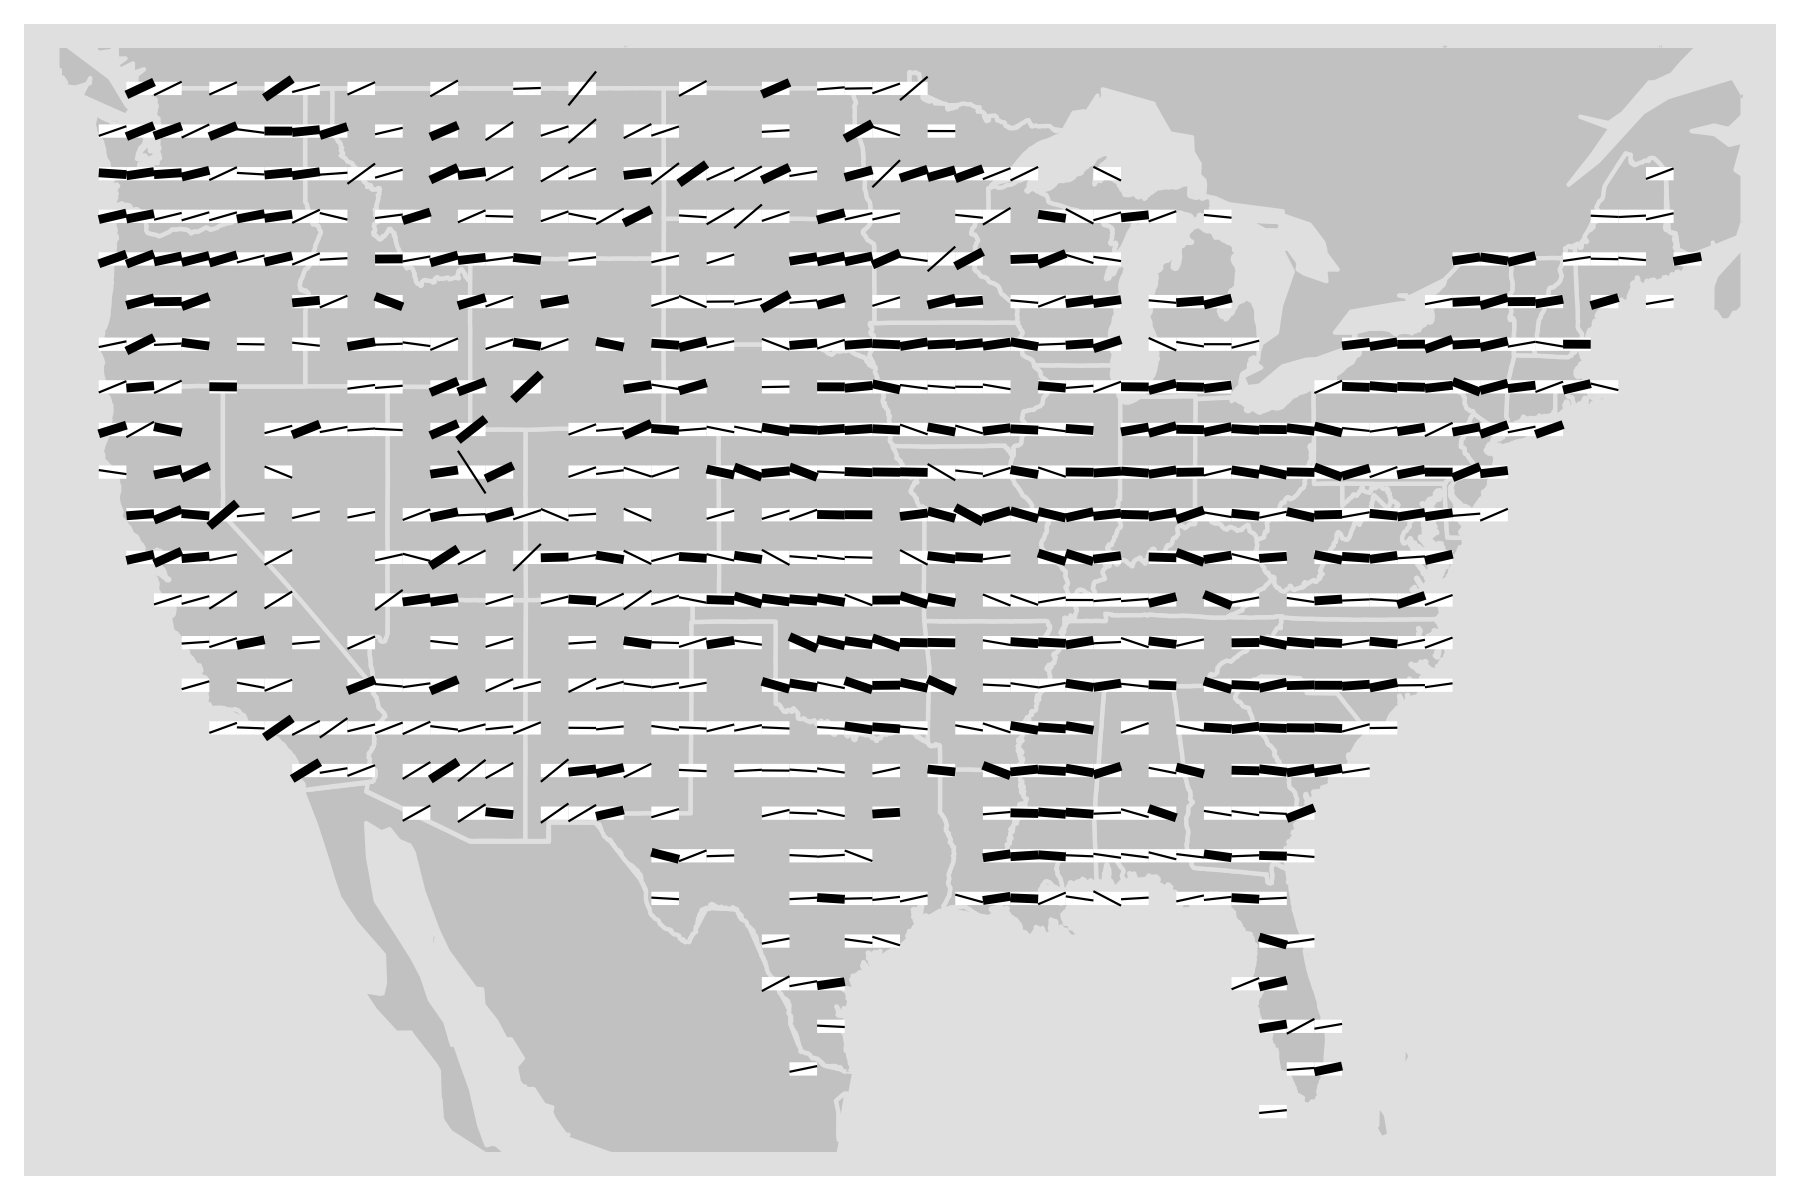
\includegraphics[width=0.5\linewidth]{usa-lin-grid}%
  \caption{Glyph-maps of seasonal patterns (left) and linear trends (right) of USHCN stations, 1950--2010.  Station locations have been rounded to the nearest degree Each location has a glyph in the seasonal plot and color of the tiles corresponds to the average temperature of the locations (red=warm, blue=cool).  Heavy lines in the linear trend plot correspond to average trends over more than one location.}
  \label{fig:irregular-grid}
\end{figure}

Reference guides become especially important in the irregular location case. Comparisons are harder in this case, as the ability to easily compare icons along a common baseline, be it along a row or column of glyphs, is absent. Without reference it is hard to tell if short series are missing data at the start or end.  

\section{Conclusions}

We have only scratched the surface of the potential of this type of display for climate data. Glyph-maps are not limited to time series plots. They are readily generalized to use any other type of display as an icon. Figure~\ref{fig:cloud} shows scatterplots as icons: temperature values are displayed horizontally and high-cloud values are displayed vertically, both locally scaled. The bivariate relationship between the two variables is explored spatially, and it is clear that it is different across the region. The equatorial Pacific and Caribbean have positive association between temperature and high cloud, while the south American continent has negative association. The second plot displays a loess curve fit to the data instead of the individual points, sharpening the view of association. Another option is available in Gauguin \citep{gribov:2006}, a icon based on a histogram, giving small univariate distribution displays for each location.

\begin{figure}[htbp]
  \centering
  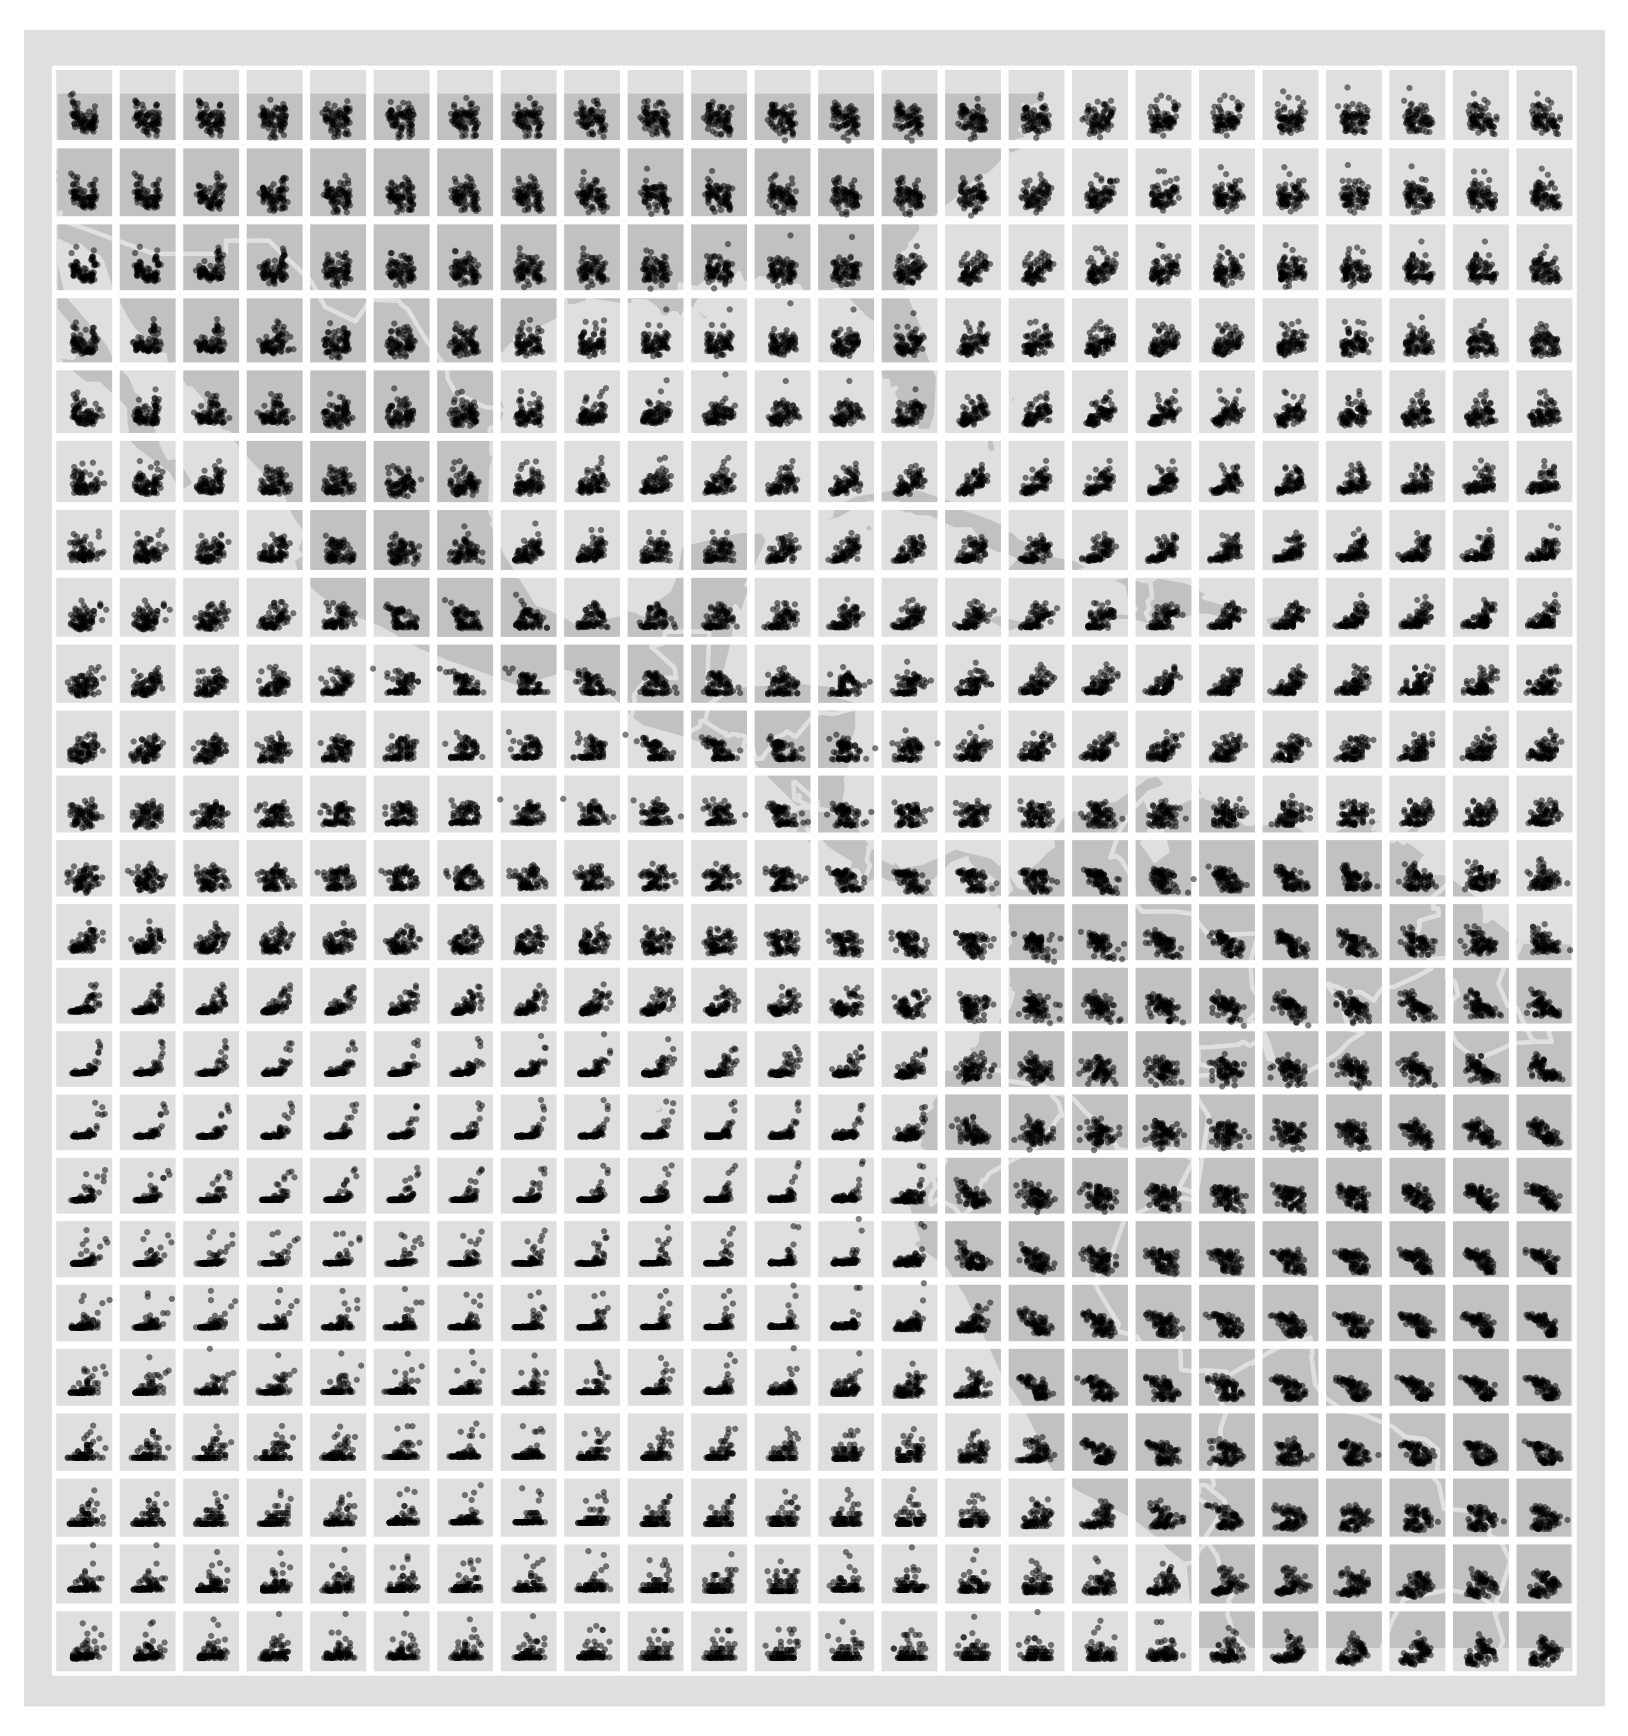
\includegraphics[width=0.5\linewidth]{nasa-scat-glyph}%
  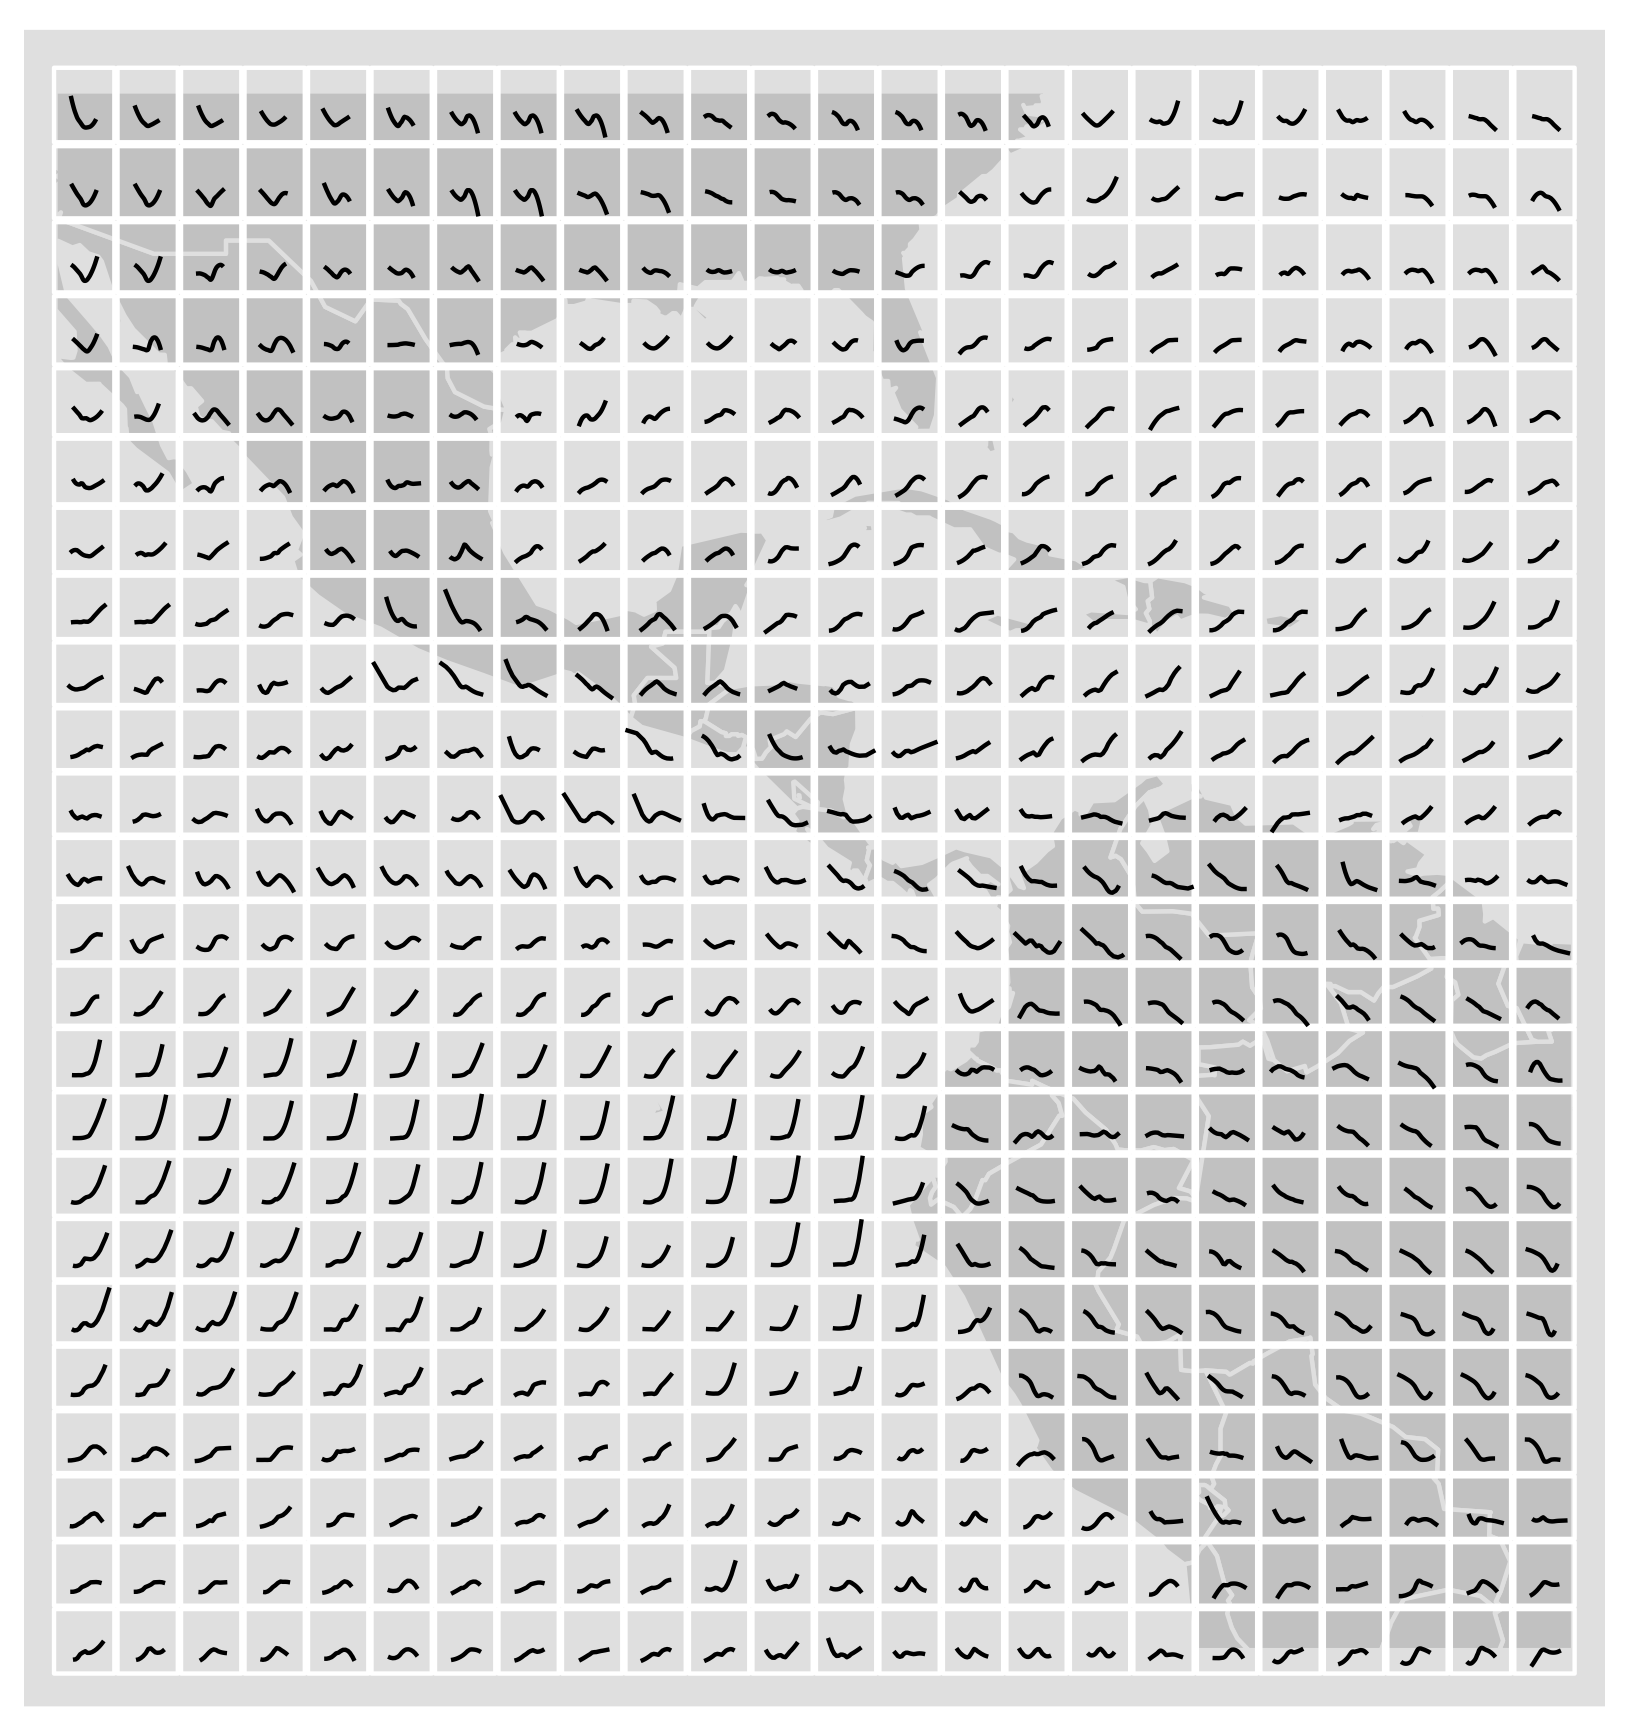
\includegraphics[width=0.5\linewidth]{nasa-loess-glyph}

  \caption{Glyph-map showing (left) scatterplot of temperature vs high-cloud and (right) smoothed (loess) curve fit to each location. The relationship between these two variables varies considerably over the spatial domain. }
  \label{fig:cloud}
\end{figure}

There is also much work to be done on the perceptual underpinnings of these displays. We have noticed that periodic trends are easier to perceive in star-glyphs, and long-term trends in line-glyphs. Is this always the case? Are their certain types of periodicity that are particularly easy to spot? These questions need to be answered with rigorous perceptual studies to help guide the use of these plots.

\bibliography{references}

\end{document}